%\documentclass[a4paper,10pt]{article}
\documentclass{iiufrgs}
\usepackage[utf8]{inputenc}
\usepackage{enumitem}
\usepackage{url}
\usepackage{setspace}
%\usepackage[list-style=extra-tabular]{acro} %problema quebra de pagina
\usepackage{longtable}
\usepackage{acro}
\acsetup{
  list-style=longtable,
}
\usepackage{graphicx}
%\usepackage[brazilian]{babel}
\usepackage{floatrow}
\usepackage{listings}
  
\setdescription{topsep=1em,parsep=0pt,partopsep=0pt,itemsep=0pt}
\setitemize{topsep=1em,parsep=0pt,partopsep=0pt,itemsep=0pt}
\setenumerate{topsep=1em,parsep=0pt,partopsep=0pt,itemsep=0pt}
%tamanho das tabelas
\DeclareFloatFont{scriptsize}{\scriptsize}% "scriptsize" is defined by floatrow, "scriptsize" not
\floatsetup[table]{font=scriptsize}
\floatsetup[longtable]{font=normalsize} % acronimos
%para notas de rodape nao quebrar com mais de 2 linhas
\interfootnotelinepenalty=10000

%capa
\course{\cgcc}
\title{Implementação de alta disponibilidade em uma empresa prestadora de serviços para Internet}
\author{Emer}{Bruno}
\advisor[]{Martinotto}{André Luis}
\location{Caxias do Sul}{}
\bibpunct{(}{)}{;}{a}{,}{,}

%declaracoes siglas
\DeclareAcronym{TI}{
  short = TI,
  long  = Tecnologia da Informação,
  class = abbrev
}
\DeclareAcronym{ECC}{
  short = ECC,
  long  = \textit{Error correction code},
  class = abbrev
}
\DeclareAcronym{RAID}{
  short = RAID,
  long  = \textit{Redundant array of independent disks},
  class = abbrev
}
\DeclareAcronym{SPOF}{
  short = SPOF,
  long  = \textit{Single point of failure},
  class = abbrev
}
\DeclareAcronym{MTBF}{
  short = MTBF,
  long  = \textit{Mean time between failures},
  class = abbrev
}
\DeclareAcronym{MTTR}{
  short = MTTR,
  long  = \textit{Mean time to repair},
  class = abbrev
}
\DeclareAcronym{SLA}{
  short = SLA,
  long  = \textit{Service level agreement},
  class = abbrev
}
\DeclareAcronym{VM}{
  short = VM,
  long  = \textit{Virtual machine},
  class = abbrev
}
\DeclareAcronym{OS}{
  short = OS,
  long  = \textit{Operating system},
  class = abbrev
}
\DeclareAcronym{PC}{
  short = PC,
  long  = \textit{Personal computer},
  class = abbrev
}
\DeclareAcronym{JVM}{
  short = JVM,
  long  = \textit{Java virtual machine},
  class = abbrev
}
\DeclareAcronym{VMM}{
  short = VMM,
  long  = \textit{Virtual machine monitor},
  class = abbrev
}
\DeclareAcronym{ISA}{
  short = ISA,
  long  = \textit{Instruction set architecture},
  class = abbrev
}
\DeclareAcronym{IVT}{
  short = IVT,
  long  = \textit{Intel virtualization technology},
  class = abbrev
}
\DeclareAcronym{AMD-V}{
  short = AMD-V,
  long  = \textit{AMD virtualization},
  class = abbrev
}
\DeclareAcronym{KVM}{
  short = KVM,
  long  = \textit{Kernel-based Virtual Machine},
  class = abbrev
}
\DeclareAcronym{JIT}{
  short = JIT,
  long  = \textit{Just-in-time},
  class = abbrev
}
\DeclareAcronym{DNS}{
  short = DNS,
  long  = \textit{Domain name system},
  class = abbrev
}
\DeclareAcronym{NAT}{
  short = NAT,
  long  = \textit{Network address translation},
  class = abbrev
}
\DeclareAcronym{IPv6}{
  short = IPv6,
  long  = \textit{Internet protocol version 6},
  class = abbrev
}
\DeclareAcronym{WHM}{
  short = WHM,
  long  = \textit{WebHost manager},
  class = abbrev
}
\DeclareAcronym{PRTG}{
  short = PRTG,
  long  = \textit{Paessler router traffic grapher},
  class = abbrev
}
\DeclareAcronym{ADSL}{
  short = ADSL,
  long  = \textit{Asymmetric Digital Subscriber Line},
  class = abbrev
}
\DeclareAcronym{PPPoE}{
  short = PPPoE,
  long  = \textit{Point-to-point protocol over ethernet},
  class = abbrev
}
\DeclareAcronym{API}{
  short = API,
  long  = \textit{Application programming interface},
  class = abbrev
}
\DeclareAcronym{LTS}{
  short = LTS,
  long  = \textit{Long term support},
  class = abbrev
}
\DeclareAcronym{FTP}{
  short = FTP,
  long  = \textit{File transfer protocol},
  class = abbrev
}
\DeclareAcronym{NRPE}{
  short = NRPE,
  long  = \textit{Nagios remote plugin executor},
  class = abbrev
}
\DeclareAcronym{SVN}{
  short = SVN,
  long  = \textit{Subversion},
  class = abbrev
}
\DeclareAcronym{PHP}{
  short = PHP,
  long  = \textit{Personal Home Page},
  class = abbrev
}
\DeclareAcronym{ASP}{
  short = ASP,
  long  = \textit{Active Server Pages},
  class = abbrev
}
\DeclareAcronym{SMTP}{
  short = SMTP,
  long  = \textit{Simple mail transfer protocol},
  class = abbrev
}
\DeclareAcronym{POP}{
  short = POP,
  long  = \textit{Post office protocol},
  class = abbrev
}
\DeclareAcronym{IMAP}{
  short = IMAP,
  long  = \textit{Internet message access protocol},
  class = abbrev
}
\DeclareAcronym{XMPP}{
  short = XMPP,
  long  = \textit{Extensible messaging and presence protocol},
  class = abbrev
}
\DeclareAcronym{SSH}{
  short = SSH,
  long  = \textit{Secure shell},
  class = abbrev
}
\DeclareAcronym{IP}{
  short = IP,
  long  = \textit{Internet protocol},
  class = abbrev
}
\DeclareAcronym{IIS}{
  short = IIS,
  long  = \textit{Internet information services},
  class = abbrev
}
\DeclareAcronym{DRBD}{
  short = DRBD,
  long  = \textit{Distributed replicated block device},
  class = abbrev
}
\DeclareAcronym{SNMP}{
  short = SNMP,
  long  = \textit{Simple Network Management Protocol},
  class = abbrev
}
\DeclareAcronym{MAC}{
  short = MAC,
  long  = \textit{Media access control},
  class = abbrev
}
\DeclareAcronym{TCP}{
  short = TCP,
  long  = \textit{Transmission control protocol},
  class = abbrev
}
\DeclareAcronym{UDP}{
  short = UDP,
  long  = \textit{User datagram protocol},
  class = abbrev
}
\DeclareAcronym{CRM}{
  short = CRM,
  long  = \textit{Cluster resource management},
  class = abbrev
}



\begin{document}

\maketitle

\begin{titlepage}
%\setcounter{page}{2} - Inclui o número da página
%\thispagestyle{headings}
\vfill

\begin{center}
{\setlength{\unitlength}{1cm}\makebox(12,6.5){\parbox[c]{12cm}{\setlength{\parskip}{0.8cm}\center\vskip -1.2cm\LARGE{\bf Implementação de alta disponibilidade em uma empresa prestadora de serviços para Internet}\par \normalsize por\par \large Bruno Emer\par}}}
\end{center}

{\large Projeto de Diplomação submetido ao curso de Bacharelado em Ciência da Computação do Centro de Ciências Exatas e da Tecnologia da Universidade de Caxias do Sul, como requisito obrigatório para graduação.}

\vfill

\begin{center}
{\Large\bf Projeto de Diplomação}
\end{center}

\vfill

\begin{singlespace}
Orientador: {André Luis Martinotto\par}

Banca examinadora:\par
\hspace{1cm} {\setlength{\unitlength}{1cm}
\makebox(9,1){\parbox[c]{9cm}{\center Maria de Fatima Webber do Prado Lima\\ CCTI/UCS}}}\par
\hspace{1cm} {\setlength{\unitlength}{1cm}
\makebox(9,1){\parbox[c]{9cm}{\center Ricardo Vargas Dorneles\\ CCTI/UCS}}}\par

\vfill

\hfill{\setlength{\unitlength}{1cm}\makebox(9,2.5){\parbox[c]{9cm}{\setlength{\parskip}{0.8cm}\center\vskip -1.2cm Projeto de Diplomação apresentado em\\ x de julho de 2016\par Daniel Luís Notari\\ Coordenador}}}

\end{singlespace}

\end{titlepage}


\tableofcontents

\chapter*{Lista de siglas}
\printacronyms[include-classes=abbrev,name=]

%\chapter*{Lista de acrônimos}
%\begin{acronym}[XXXXXXXXXX]
%\acro{API}[\textit{API}]{\textit{Application Programming Interface}}
%\end{acronym}

\listoffigures
\listoftables

\keyword{Alta disponibilidade}
\keyword{Virtualização}
\keyword{Tolerância a falhas}
\keyword{Código aberto}

\begin{abstract}

O número de serviços oferecidos através da Internet vem crescendo a cada dia que passa. Sendo assim, a alta disponibilidade é um fator
crucial para empresas que prestam este tipo de serviço. De fato, o aumento da disponibilidade é um grande diferencial para essas empresas.

Dentro deste contexto, neste trabalho é feito um estudo para a implementação de um ambiente de alta disponibilidade em uma empresa prestadora 
de serviços para Internet, utilizando ferramentas de código aberto. Para isso, foi feita uma análise dos serviços oferecidos pela empresa, bem 
como um levantamento do ambiente de servidores da mesma.

Criou-se um projeto de implementação para a solução de alta disponibilidade no ambiente da empresa, esse ambiente utiliza virtualização para uma 
grande parte dos serviços. Para tal, pesquisou-se algumas ferramentas de gerenciamento de \textit{cluster} e de replicação de dados. A partir 
destas ferramentas é feita uma análise das mesmas e adotada a mais adequada para o ambiente da empresa. Deste modo, o \textit{cluster} é composto 
pelo \textit{software} \textit{Pacemaker}, que faz o gerenciamento do \textit{cluster} e pelo \textit{software} \textit{DRBD}, que é responsável 
pela replicação dos dados.

Por fim validou-se o ambiente de alta disponibilidade através de testes que simulam falhas de \textit{hardware}, de energia elétrica e de
\textit{software}. Além disso, simulou-se manutenções e reinicializações do servidores físicos sem causar indisponibilidade dos serviços.

\end{abstract}

\begin{englishabstract}{}{high availability, virtualization, fault tolerance, open source}

The number of services provided through the Internet come growing each passed day. Thus, high availability is a crucial factor to the 
companies that provide this kind of service. In fact, the availability growth is a great differential for these companies.

Within this context, in this article was done a study to do a implementation of a high availability environment in a company that provide 
Internet services, making use? at open source tools. For this?, was done a analisys? of services provide by the company, 
? a ? its servers environment.

A implementation project was created for a high availability solution at company environment, this company uses virtualization to the biggest?
among of its services. ?, was done a research some tools to cluster manage and to data replication?. With this tools was analisado? and adopted?
the most adequada? tool to the company environment. ?, the cluster was ? by software Pacemaker, that is the cluster manager, and by software
DRBD, that is the data replication software.

? was validated? the high availability environment through at tests that simulate hardware fails, energy fails and software fails. 
In addition, was simulated maintenance and reboot of physical servers with cause unavailability of the services.

??

\end{englishabstract}


%includes
\chapter{Introdução}
O crescente avanço tecnológico e o desenvolvimento da Internet, provocou um aumento no número de aplicações ou serviços que dependem da 
infraestrutura de \ac{TI}. Além disso, percebe-se um aumento significativo no número de operações \textit{on-line} que são realizadas, 
tanto por organizações públicas ou privadas, quanto por grande parte da população.

Desta forma, a sociedade está cada vez mais dependente da tecnologia, de computadores e de sistemas. De fato, pode-se observar 
sistemas computacionais desde em uma farmácia, até em uma grande indústria. Sendo assim, a estabilidade e a disponibilidade desses 
sistemas apresenta um grande impacto em nosso dia-a-dia, pois um grande número de atividades cotidianas dependem deles.

Uma interrupção imprevista em um ambiente computacional poderá causar um prejuízo financeiro para a empresa que fornece o serviço, 
além de interferir na vida das pessoas que dependem de forma direta ou indireta deste serviço. 
Essa interrupção terá maior relevância para as corporações cujo o serviço ou produto final é fornecido através da Internet, 
como por exemplo, o comércio eletrônico, \textit{web sites}, sistemas corporativos, entre outros. 
Em um ambiente extremo, pode-se imaginar o caos e o possível risco de perda de vidas que ocorreria em caso de uma falha 
em um sistema de controle aéreo \cite{costa2009}.

Para essas empresas um plano de contingência é fundamental para garantir uma boa qualidade de serviço, além de otimizar o desempenho 
das atividades, e também para fazer uma prevenção de falhas e uma recuperação rápida caso essas ocorram \cite{costa2009}.
De fato, hoje em dia a confiança em um serviço é um grande diferencial para a empresa fornecedora deste, 
sendo que a alta disponibilidade é fundamental para atingir este objetivo.

A alta disponibilidade consiste em manter um sistema disponível por meio da tolerância a falhas, isto é, utilizando mecanismos que fazem a 
detecção, mascaramento e a recuperação de falhas, sendo que esses mecanismos podem ser implementados a nível de \textit{software} ou de 
\textit{hardware} \cite{reis2009}. Para que um sistema seja altamente disponível ele deve ser tolerante a falhas, sendo que a tolerância
a falhas é, frequentemente, implementada utilizando redundância. No caso de uma falha em um dos componentes evita-se a interrupção do sistema,
uma vez que o sistema poderá continuar funcionando utilizando o outro componente \cite{batista2007}.

Neste trabalho será realizado um estudo sobre a implementação de um sistema de alta disponibilidade em uma empresa prestadora de serviços para 
Internet. Essa empresa oferece serviços, como por exemplo hospedagens de sites, \textit{e-mail}, sistemas de gestão, \textit{e-mail marketing}, 
entre outros. A empresa possui aproximadamente 60 servidores físicos e virtuais, e aproximadamente 9000 clientes, 
sendo que em períodos de pico atende em torno de 1000 requisições por segundo. 

Atualmente, a empresa possui redundância de conexões de acesso à Internet, refrigeração e energia, com \textit{nobreaks} e geradores. 
Porém, essa empresa não possui nenhuma redundância nos serviços que estão sendo executados nos servidores. Desta forma, caso ocorra 
uma falha de \textit{software} ou de \textit{hardware}, os serviços ficarão indisponíveis. Neste trabalho será realizada uma análise dos 
serviços oferecidos pela empresa, sendo que mecanismos de alta disponibilidade serão desenvolvidos para os serviços mais críticos. 
Para a redução dos custos serão utilizadas ferramentas gratuitas e de código aberto.

\section{Objetivos}
Atualmente a empresa estudada não possui nenhuma solução de alta disponibilidade para seus serviços críticos. Desta forma, neste trabalho 
será desenvolvida uma solução de alta disponibilidade para estes serviços, sendo que essa solução será baseada no uso de ferramentas de 
código aberto e de baixo custo. Para que o objetivo geral seja atendido os seguintes objetivos específicos deverão ser realizados:

\begin{itemize}
\item Identificar os serviços críticos a serem integrados ao ambiente de alta disponibilidade;
\item Definir as ferramentas a serem utilizadas para implementar tolerância a falhas;
\item Realizar testes para a validação do sistema de alta disponibilidade que foi desenvolvido.
\end{itemize}

\section{Estrutura do trabalho}
O trabalho foi estruturado em cinco capítulos, que são:

\begin{itemize}
 \item Capítulo \ref{cap:altadisponibilidade}: apresenta o conceito de alta disponibilidade e conceitos relacionados;
 \item Capítulo \ref{cap:virtualizacao}: é apresentado um breve histórico da virtualização, bem como o conceito de máquinas virtuais e as 
 estratégias utilizadas para a implementação das mesmas;
 \item Capítulo \ref{cap:estudodecaso}: descreve o ambiente atual da empresa com os serviços que são fornecidos;
 \item Capítulo \ref{cap:projetoimplementacao}: neste capítulo são descritos os serviços críticos e é apresentado a solução de alta disponibilidade 
 proposta. Essa proposta de solução foi desenvolvida baseada na utilização de virtualização;
 \item Capítulo \ref{cap:conclusao}: apresenta as conclusões parciais do trabalho e o cronograma de andamento.
\end{itemize}

\chapter{Alta disponibilidade}
\label{cap:altadisponibilidade}

Alta disponibilidade é uma conhecida técnica que está sendo cada vez mais empregada em ambientes computacionais. O objetivo de prover
alta disponibilidade resume-se em garantir que um serviço esteja sempre disponível quando o cliente solicitar ou acessar \cite{costa2009}.
A alta disponibilidade geralmente é implementada com uma redundância de \textit{hardware} ou de \textit{software}, sendo que quanto maior for 
a disponibilidade desejada maior deverá ser a redundância no ambiente, assim reduzindo os pontos únicos de falha, que em inglês são chamados 
de \ac{SPOF}. A alta disponibilidade está diretamente relacionada aos conceitos de: 
\begin{itemize}
 \item Dependabilidade: indica a qualidade do serviço fornecido e a confiança depositada neste serviço. A dependabilidade envolve atributos 
 como segurança de funcionamento, segurança de acesso, manutenabilidade, testabilidade e comprometimento com o desempenho \cite{weber2002};
 \item Confiabilidade: é o atributo mais importante, pois transmite a ideia de continuidade de serviço \cite{pankaj1994}. A confiabilidade 
 refere-se a probabilidade de um serviço estar funcionando corretamente durante um dado intervalo de tempo;
 \item Disponibilidade: é a probabilidade de um serviço estar operacional no instante em que for solicitado \cite{costa2009};
 \item Tolerância a falhas: procura garantir a disponibilidade de um serviço utilizando mecanismos capazes de detectar, mascarar e recuperar 
 falhas. O seu principal objetivo é alcançar a dependabilidade, assim indicando uma boa qualidade de serviço \cite{costa2009}. A tolerância a 
 falhas é um dos principais conceitos da alta disponibilidade, sendo descrita na Seção \ref{section:toleranciafalhas}.
\end{itemize}

\section{Tolerância a falhas}
\label{section:toleranciafalhas}

Sabe-se que o \textit{hardware} tende a falhar, principalmente devido a fatores físicos, por isso utiliza-se métodos para a prevenção 
de falhas. A abordagem de prevenção de falhas é realizada na etapa de projeto, ou seja, consiste em definir mecanismos que impeçam que 
que as falhas ocorram. Além disso, a prevenção de falhas melhora a disponibilidade e a confiabilidade de um serviço, uma vez que esta 
tem como objetivo diminuir a possibilidade de falhas antes de colocar o sistema em uso.

A prevenção de falhas não eliminará todas as possíveis falhas. Sendo assim, a tolerância a falhas procura fornecer a disponibilidade de 
um serviço mesmo com a presença de falhas. De fato, enquanto a prevenção de falhas tem foco nas fases de projeto, teste e validação, a 
tolerância a falhas apresenta como foco a utilização de componentes replicados para mascarar as falhas \cite{pankaj1994}.

O objetivo da tolerância a falhas é aumentar a disponibilidade de um sistema, ou seja, aumentar o intervalo de tempo em que os serviços 
fornecidos estão disponíveis aos usuários. Um sistema é dito tolerante a falhas se ele for capaz de mascarar a presença de falhas ou recuperar-se 
de uma sem afetar o funcionamento do sistema \cite{pankaj1994}. %{pereirafilho2004}

A tolerância a falhas frequentemente é implementada utilizando redundância (Seção \ref{section:redundancia}). 
Um exemplo muito utilizado para tornar um sistema tolerante a falhas é a virtualização. Nestes ambientes normalmente existem dois servidores 
físicos onde máquinas virtuais são executadas, sendo que no caso de um dos servidores falhar, o \textit{software} de monitoramento fará a 
transferência das máquinas virtuais para o outro servidor, de forma transparente aos usuários, evitando assim a indisponibilidade do serviço. 
Os principais conceitos de virtualização, são apresentados no Capítulo \ref{cap:virtualizacao}.

A tolerância a falhas pode ser dividida em dois tipos. O primeiro tipo, o mascaramento, não se manifesta na forma de erro ao sistema, 
pois as falhas são tratadas na origem. O mascaramento é utilizado principalmente em sistemas críticos e de tempo real. Um exemplo são os 
códigos de correção de erros, em inglês \ac{ECC}, que são utilizados em memórias para a detecção e a correção de erros.

O segundo tipo de tolerância a falhas consiste em detectar, localizar a falha, e reconfigurar o \textit{software} ou \textit{hardware} de 
forma a corrigi-la. Esse tipo de tolerância a falha é dividido nas seguintes etapas \cite{weber2002}. 

\begin{itemize}
 \item Detecção: realiza o monitoramento e aguarda uma falha se manifestar em forma de erro, para então passar para a próxima fase. 
 Um exemplo de detecção de erro é um cão de guarda (\textit{watchdog timer}), que recebe um sinal do programa ou serviço que esta sendo 
 monitorado e caso este sinal não seja recebido, o \textit{watchdog} irá se manifestar na forma de erro. 
 Um outro exemplo é o esquema de duplicação e comparação, onde são realizadas operações em componentes replicados com os mesmos dados de 
 entrada, e então os dados de saída são comparados. No caso de diferenças nos dados de saída um erro é gerado.
 \item Confinamento: responsável pela restrição de um erro para que dados inválidos não se propaguem para todo o sistema, pois entre a falha e a
 detecção do erro há um intervalo de tempo. Neste intervalo pode ocorrer a propagação do erro para outros componentes do sistema, sendo assim, 
 antes de executar medidas corretivas é necessário definir os limites da propagação. Na fase de projeto essas restrições devem ser previstas
 e tratadas. Um exemplo de confinamento é o isolamento de alguns processos que estão em execução em um sistema operacional. Neste caso, o 
 sistema faz o gerenciamento dos processos para isolar e impedir que as falhas de um processo gerem problemas em outros processos.
 \item Recuperação: após a detecção de um erro ocorre a recuperação, onde o estado de erro é alterado para estado livre de erros. A recuperação
 pode ser feita de duas formas, que são:
 \begin{itemize}
  \item \textit{forward error recovery} (recuperação por avanço): ocorre uma condução para um estado que ainda não ocorreu. É a forma
  de recuperação mais eficiente, porém mais complexa de ser implementada.
  \item \textit{backward error recovery} (recuperação por retorno): ocorre um retorno para um estado anterior e livre de erros.
  Para retornar ao estado anterior podem ser utilizados pontos de recuperação (\textit{checkpoints}). Assim, quando ocorrer um erro, um 
  \textit{rollback} é executado, ou seja, o sistema retornará a um estado anterior a falha.
 \end{itemize}
 \item Tratamento: procura prevenir que futuros erros aconteçam. Nesta fase ocorre a localização da falha para descobrir o 
 componente que originou a falha. A substituição do componente danificado pode ser feita de forma manual ou automática. 
 O reparo manual é feito por um operador que é responsável pelo reparo ou substituição de um componente. Como exemplo pode-se citar
 a troca de um disco rígido de um servidor. Já o reparo automático é utilizado quando existe um componente em espera para a substituição, 
 como por exemplo, um disco configurado como \textit{hot spare}, ou seja, um componente de \textit{backup} que assumirá o lugar do 
 outro imediatamente após o componente principal falhar. Em \textit{storages} ou servidores, o \textit{hot spare} pode ser configurado 
 através de um \ac{RAID} \cite{rouse2013}.
\end{itemize}

\section{Redundância}
\label{section:redundancia}

A redundância pode ser implementada através da replicação de componentes, e apresenta como objetivo reduzir o número de \ac{SPOF} e garantir 
o mascaramento de falhas. Na prática, se um componente falhar ele deve ser reparado ou substituído por um novo, sem que haja uma 
interrupção no serviço. Além disso, a redundância pode ser implementada através do envio de sinais ou \textit{bits} de controle junto aos dados, 
servindo assim para detecção e correção de erros \cite{weber2002}. Segundo \cite{norvag2000} existem quatro tipos diferentes 
de redundância que são:
\begin{itemize}
 \item \textit{Hardware}: utiliza-se a replicação de componentes, sendo que no caso de falha em um deles o outro possa assumir seu lugar. 
 Para fazer a detecção de erros a saída de cada componente é constantemente monitorada e comparada à saída do outro componente.
 Um exemplo prático de redundância de \textit{hardware} são os servidores com fontes redundantes. Neste caso são utilizadas duas fontes 
 ligadas em paralelo, sendo que, caso uma falhe a outra suprirá a necessidade de todo o servidor;
 \item Informação: ocorre quando uma informação extra é enviada ou armazenada para possibilitar a detecção e a correção de erros.
 Um exemplo são os \textit{checksums} (soma de verificação). Esses são calculados antes da transmissão ou armazenamento dos dados 
 e recalculados ao recebê-los ou recuperá-los, assim sendo possível verificar a integridade dos dados. Outro exemplo bastante comum são os 
 \textit{bits} de paridade que são utilizados para detectar falhas que afetam apenas um \textit{bit} \cite{weber2002};
 \item \textit{Software}: pode-se definir redundância de \textit{software} como a configuração de um serviço ou \textit{software} em
 dois ou mais locais. Pode-se citar como exemplo um sistema gerenciador de banco de dados \textit{MySQL}, que pode ser configurado 
 com um modelo de replicação do tipo \textit{master-slave}, onde um servidor principal (\textit{master}) grava as operações em um arquivo, 
 para que então os servidores \textit{slaves}, possam recuperar e executar essas operações, com isso mantendo os dados sincronizados. Neste caso, 
 tanto o servidor \textit{master} quanto os \textit{slaves} executam o serviço \textit{MySQL}, caracterizando uma redundância \cite{viana201}. 
 A redundância de \textit{software} também pode ser implementada com o objetivo de tolerar falhas e \textit{bugs} em um \textit{software} 
 crítico. Existem algumas técnicas que podem ser utilizadas para isso, como por exemplo, a programação de \textit{n}-versões, que consiste 
 no desenvolvimento de \textit{n} versões de um mesmo \textit{software}. Desta forma, possibilita-se o aumento da disponibilidade, uma vez que 
 essas versões provavelmente não apresentarão os mesmos erros. A programação de \textit{n}-versões possui um custo muito elevado, não sendo muito 
 utilizada.
 \item Tempo: este é feito através da repetição de um conjunto de instruções em um mesmo componente, assim detectando uma falha caso ocorra. 
 Essa técnica necessita tempo adicional, e é utilizada em sistemas onde o tempo não é crítico. Como exemplo pode-se citar um \textit{software} 
 de monitoramento de serviços que faz um teste em cada serviço. No caso de ocorrência de uma falha em um serviço, uma ação corretiva 
 será executada para reestabelecer este serviço. Essa técnica, diferentemente da redundância de \textit{hardware}, não requer um 
 \textit{hardware} extra para sua implementação \cite{costa2009}.
\end{itemize}

\section{Cálculo da alta disponibilidade}

Um aspecto importante sobre alta disponibilidade é como medi-la. Para isso são utilizados os valores de \textit{uptime} e \textit{downtime}, 
que são respectivamente o tempo em que os serviços estão em execução e o tempo em que não estão executando. A alta disponibilidade 
pode ser expressa pela quantidade de ``noves'', isto é, se um serviço possui quatro noves de disponibilidade, este possui uma 
disponibilidade de 99,99\% \cite{pereirafilho2004}.

A Tabela \ref{tab:dispniveis} apresenta alguns níveis de disponibilidade, e os seus percentuais de \textit{Uptime} e os \textit{Downtime} por ano. 
Já na última coluna tem-se alguns exemplos de serviços relacionados ao nível de disponibilidade. Pode-se observar que para alguns serviços, 
como por exemplo, sistemas bancários ou sistemas militares é necessário um alto nível de disponibilidade \cite{pereirafilho2004}.

\begin{table}[h!]
\caption {Níveis de alta disponibilidade e exemplos de sistemas}
\label{tab:dispniveis}
\begin{center}
\begin{tabular}{|l|l|l|l|}\hline
Nível & Uptime & Downtime por ano & Exemplos\\\hline
1 & 90\% & 36,5 dias & computadores pessoais\\\hline
2 & 98\% & 7,3 dias & \\\hline
3 & 99\% & 3,65 dias & sistemas de acesso\\\hline
4 & 99,8\% & 17 horas e 30 minutos & \\\hline
5 & 99,9\% & 8 horas e 45 minutos & provedores de acesso\\\hline
6 & 99,99\% & 52,5 minutos & CPD, sistemas de negócios\\\hline
7 & 99,999\% & 5,25 minutos & sistemas de telefonia ou bancários\\\hline
8 & 99,9999\% & 31,5 minutos & sistemas de defesa militar\\\hline
\end{tabular}
\end{center}
\end{table}

A porcentagem de disponibilidade (\textit{d}) pode ser calculada através da equação
%OBS: aumenta a disponibilidade caso o tempo entre as paradas for maior
\begin{equation}
d = \frac{MTBF}{(MTBF + MTTR)}
\label{disponibilidade}
\end{equation}
onde o \ac{MTBF} corresponde ao tempo médio entre falhas, ou seja, corresponde ao tempo médio entre as paradas de um serviço. Já o \ac{MTTR} é o 
tempo médio de recuperação, isto é, o tempo entre a queda e a recuperação de um serviço \cite{goncalves2009}.

A alta disponibilidade é um dos principais fatores que fornece confiança aos clientes ou usuários de um serviço, sendo extremante importante 
em empresas que fornecem serviços \textit{on-line}. Por isso, as empresas desenvolveram o \ac{SLA}, que é um acordo de nível de serviço, 
o qual garante que o serviço fornecido atenda as expectativas dos clientes. Um \ac{SLA} é um documento contendo uma descrição e uma definição 
das características mais importantes do serviço que será fornecido. Esse acordo apresenta ainda o percentual de disponibilidade do serviço.
Além disso, um \ac{SLA} deverá conter descrição do serviço, requerimentos, horário de funcionamento, \textit{uptime} do serviço, 
\textit{downtime} máximo do serviço, entre outros \cite{smith2010}.

\section{Considerações finais}

Neste capítulo foram descritos os principais conceitos de alta disponibilidade e conceitos relacionados. Como mencionado anteriormente, 
um dos principais recursos utilizados para a obtenção de alta disponibilidade é a virtualização, uma vez que essas são utilizadas para 
implementar a redundância de \textit{software}. Desta forma, no próximo capítulo será feita uma breve definição de virtualização, 
com as vantagens e as estratégias de implementação de máquinas virtuais.

\chapter{Virtualização}
\label{cap:virtualizacao}

O conceito virtualização surgiu na década de 60, onde o usuário muitas vezes necessitava de um ambiente individual, 
com suas próprias aplicações e totalmente isolado dos demais usuários. Esse foi um dos principais motivos para a criação das máquinas 
virtuais, que na época eram conhecidas como \ac{VM}. As \ac{VM}s apresentaram uma forte expansão com o sistema operacional \textit{370}, que foi 
desenvolvido pela \textit{IBM}, e foi um dos principais sistemas comerciais com suporte à virtualização da época. Esse sistema operacional 
era executado em \textit{mainframes}, que eram grandes servidores capazes de processar um grande volume de informações \cite{laureano2008}. 

Na década de 80 houve uma redução no uso da virtualização devido a popularização do \ac{PC}. Na época era mais vantajoso disponibilizar 
um \ac{PC} para cada usuário do que investir em \textit{mainframes}. Devido à crescente melhora na performance do \ac{PC} e
ao surgimento da linguagem \textit{Java}, no início da década de 90, a tecnologia de virtualização retornou com o conceito de virtualização
de aplicação \cite{laureano2008}.

A virtualização foi definida nos anos 60 e 70 como uma camada entre o \textit{hardware} e o sistema operacional que possibilitava a 
divisão e a proteção dos recursos físicos. Porém, atualmente ela abrange outros conceitos, como por exemplo a \ac{JVM}, que não virtualiza
um \textit{hardware}. De fato, a \ac{JVM} permite que uma aplicação convidada execute em diferentes tipos de sistemas operacionais.

Atualmente, define-se virtualização como uma camada de \textit{software} que utiliza os serviços fornecidos por uma determinada interface de 
sistema para criar outra interface de mesmo nível. Assim, a virtualização permite a comunicação entre interfaces distintas, de forma que uma 
aplicação desenvolvida para uma plataforma \textit{X} possa também executar em uma plataforma \textit{Y} \cite{laureano2008}.

Como mencionado, a virtualização permite a comunicação entre diferentes interfaces, sendo que existem diferentes tipos de interfaces
nos sistemas de computação \cite{maziero2013}:
\begin{itemize}
 \item Conjunto de instruções ou \ac{ISA}: é a interface básica, que fica entre o \textit{software} e o \textit{hardware}, e é composta por 
 instruções de código de máquina. Essa interface é dividida em dois grupos:
 \begin{itemize}
  \item Instruções de usuário ou \textit{User \ac{ISA}}: são instruções disponíveis à aplicações de usuários. Essas instruções executam em 
  modo usuário, sendo que neste modo existem restrições que procuram garantir um controle e segurança no acesso aos recursos de \textit{hardware}. 
  Instruções de usuário são instruções não privilegiadas, ou seja, são instruções que podem ser executadas sem interferir em outras tarefas, 
  porque elas não acessam recursos compartilhados. Este grupo de interface contém, por exemplo, instruções de operações aritméticas e instruções 
  de ponto flutuante \cite{buyya2013};
  %Caso uma instrução privilegiada for executada no modo usuário, ela manifesta-se através de uma interrupção e será devidamente tratada;
  \item Instruções de sistema ou \textit{System \ac{ISA}}: essas instruções geralmente são disponibilizadas para o núcleo do sistema operacional. 
  Elas são instruções privilegiadas, ou seja, são instruções que acessam recursos compartilhados. Essas instruções são executadas em modo 
  supervisor (ou modo \textit{kernel}), que permite realizar operações sensíveis\footnote[1]{Operações sensíveis são instruções que podem alterar o 
  estado do processador.} no \textit{hardware} \cite{buyya2013}. Como exemplo de instruções de sistema pode-se citar as instruções que alteram 
  o estado dos registradores do processador; % entrada e saída (E/S)
 \end{itemize}
 \item Chamadas de sistema ou \textit{syscalls}: são operações oferecidas pelo núcleo do sistema operacional para as aplicações dos usuários.
 Essas operações permitem um acesso controlado aos dispositivos, a memória e ao processador. 
 As instruções privilegiadas não podem ser executadas no modo usuário, por isso, as aplicações de usuários utilizam chamadas de sistemas em seu 
 lugar, e então o sistema operacional determina se essas operações poderão comprometer ou não a integridade do sistema \cite{marinescu2013}.
 Um exemplo de chamada de sistema é uma operação de escrita em disco rígido ou qualquer operação de entrada e saída feita por aplicações de usuários.
\end{itemize}

A Figura \ref{fig:interfaces_isa} mostra as diferentes interfaces entre aplicações de usuários, bibliotecas, núcleo do sistema operacional e o 
\textit{hardware}.

\begin{figure}[h!]
 \centering
 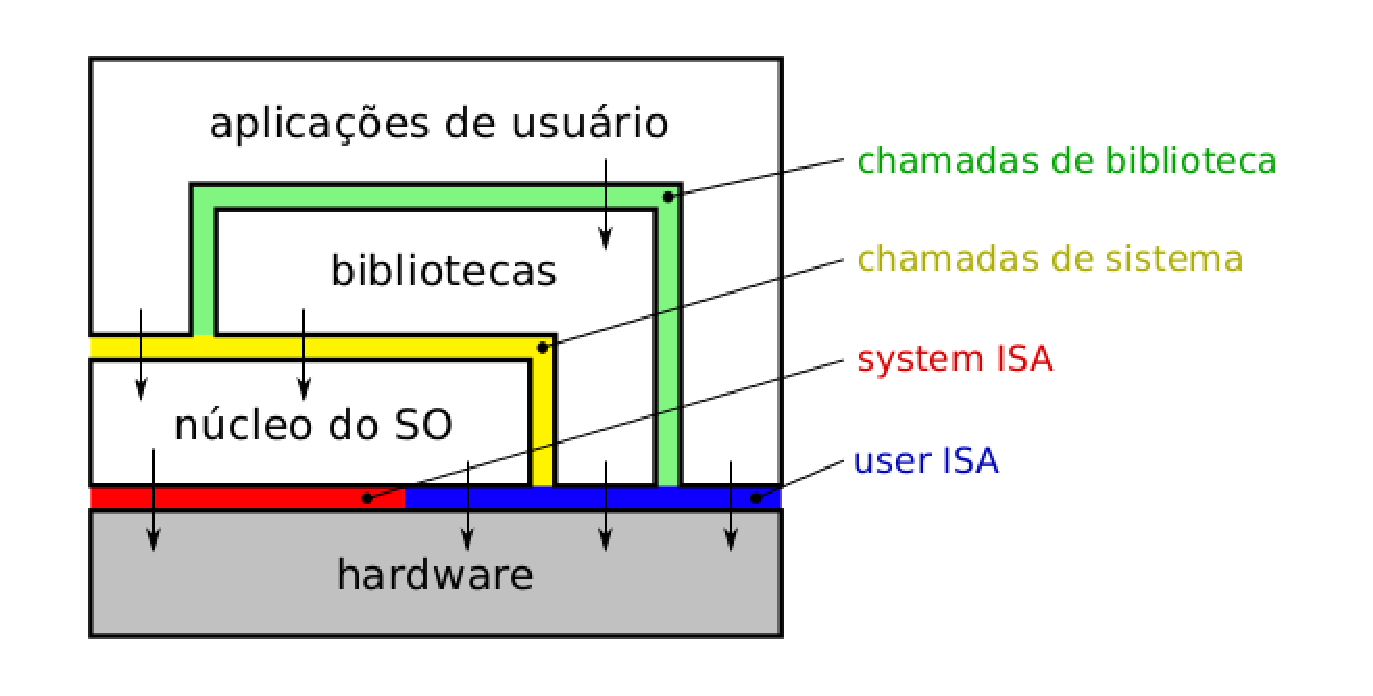
\includegraphics[width=300px]{img/interfaces_isa.eps}
 \caption{Interfaces de sistemas de computação.}
 \label{fig:interfaces_isa}
 Fonte: \citet{maziero2013}
\end{figure}

Máquinas virtuais podem ser divididas em dois grupos principais, que são: as máquinas virtuais de aplicação (Seção \ref{section:virtaplicacao}), 
e máquinas virtuais de sistema (Seção \ref{section:virtsistema}). As máquinas virtuais de aplicação fazem a virtualização de uma aplicação e 
suportam apenas uma aplicação, ou seja, elas provêm um ambiente que permite a execução de uma aplicação convidada. Um exemplo de máquina 
virtual de aplicação é a \ac{JVM}. Já uma máquina virtual de sistema suporta um sistema operacional convidado, com suas aplicações executando 
sobre ele. Uma máquina virtual executando sobre o hipervisor \ac{KVM} é um exemplo de máquina virtual de aplicação \cite{laureano2008}.

Na Figura \ref{fig:vms_tipos} (a) tem-se o modelo de máquina virtual de aplicação, onde uma \ac{JVM}, juntamente com aplicações, está executando 
sobre um sistema operacional hospedeiro. A Figura \ref{fig:vms_tipos} (b) apresenta uma máquina virtual de sistema, que possui dois sistemas 
operacionais executando sobre um único \textit{hardware} por meio do hipervisor.

\begin{figure}[h!]
 \centering
 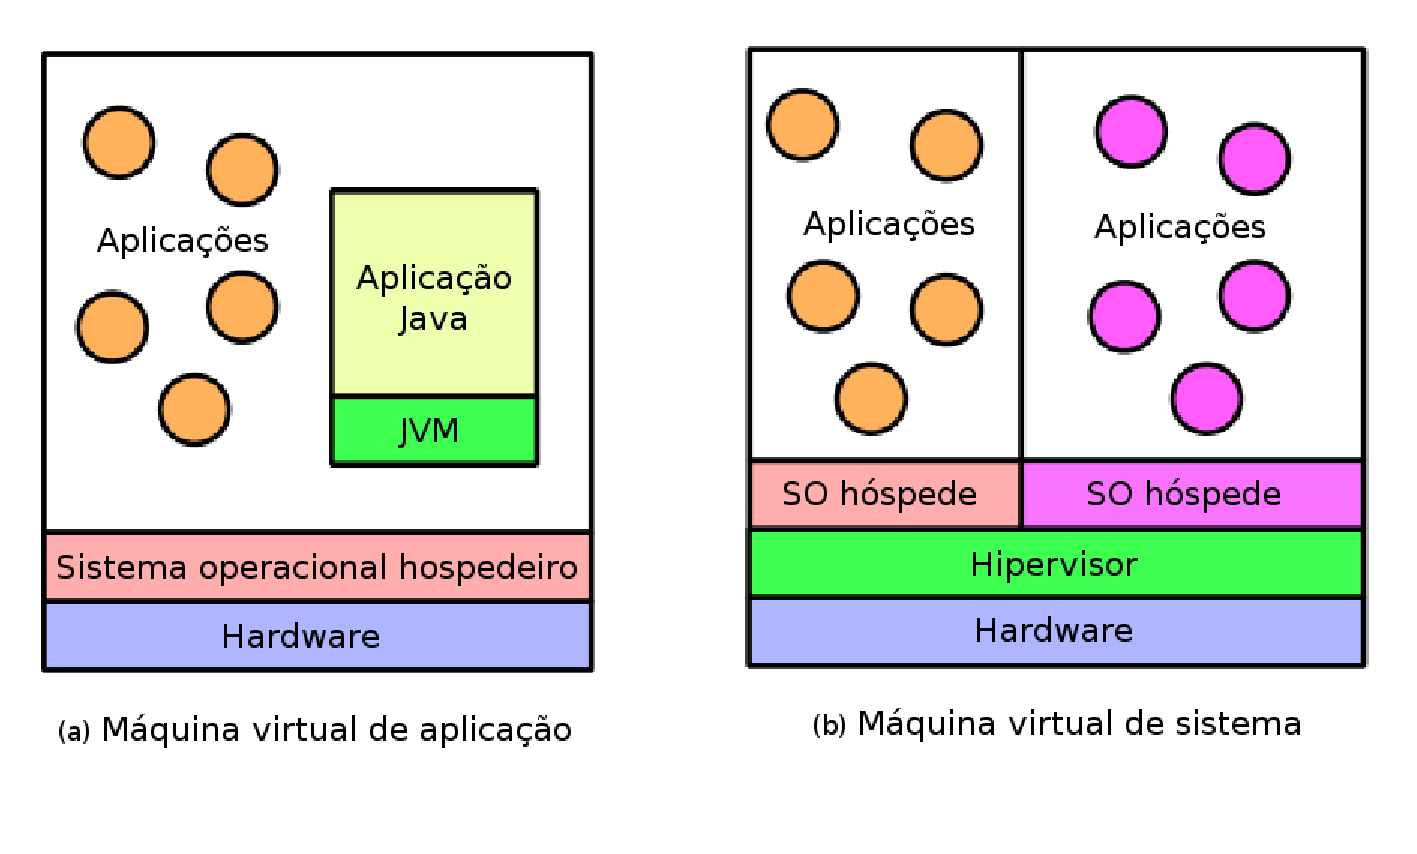
\includegraphics[width=420px]{img/vms_tipos.eps}
 \caption{Máquinas virtuais de aplicação e de sistema.}
 \label{fig:vms_tipos}
 Fonte: \citet{laureano2008}
\end{figure}

\section{Máquinas virtuais de aplicação}
\label{section:virtaplicacao}

As máquinas virtuais de aplicação, também chamadas de máquinas virtuais de processos, são responsáveis por prover um ambiente que permite 
a execução de uma aplicação convidada, sendo que esta aplicação possui um conjunto de instruções, ou de chamadas de sistema, diferentes da 
arquitetura do sistema hospedeiro. Neste caso, quando temos uma chamada de sistema ou instruções de máquina, será necessário uma 
tradução dessas interfaces, que será feita pela camada de virtualização. Os dois principais tipos de máquinas virtuais de aplicação são:

\begin{itemize}
 \item Máquinas virtuais de linguagem de alto nível: esse tipo de máquina virtual foi criado levando em consideração uma linguagem de 
 programação e o seu compilador. Neste caso, o código compilado gera um código intermediário que não pode ser executado em uma arquitetura real, 
 mas pode ser executado em uma máquina virtual. Sendo assim, para cada arquitetura ou sistema operacional deverá existir uma máquina virtual que
 permita a execução da aplicação. Como exemplo deste tipo de máquina virtual pode-se citar a máquina virtual Java (\ac{JVM})
 e a \textit{Microsoft Common Language Infrastructure}, que é a base da plataforma \textit{.NET} \cite{carissimi2008};
 \item Emulação do sistema operacional: nesse caso é feito um mapeamento entre as chamadas de sistema que são utilizadas pela aplicação 
 e as chamadas de sistema operacional hospedeiro. A virtualização de aplicação pode ser encontrada em ferramentas que emulam uma aplicação que foi
 desenvolvida para uma plataforma em uma outra plataforma. Como exemplo, pode-se citar o \textit{Wine} \cite{wine}, que permite executar 
 aplicações \textit{Windows} em plataformas \textit{Linux}.
\end{itemize}

%Na virtualização de aplicação também existem máquinas virtuais que utilizam as mesmas interfaces \ac{ISA} do computador real,
%com isso uma grande parte das instruções podem ser executadas diretamente, com exceção de instruções privilegiadas, que serão devidamente
%tratadas. Alguns tipos de máquinas virtuais de aplicação que utilizam as interfaces do sistema real são:

%\begin{itemize}
% \item Sistemas operacionais multitarefas: sistemas operacionais que suportam simultaneamente mais de um usuário também podem ser
% vistos como máquinas virtuais. Em um sistema multitarefa cada processo possui um ``processador virtual'' (devido a rápida troca de 
% contextos do processador real), uma ``memória virtual'' (memória alocada para o processo) e outros recursos que podem ser acessados
% através de chamadas de sistema;
% \item Tradutores dinâmicos: esses tradutores analisam e otimizam o código de máquina para torná-lo mais eficiente. Essa otimização 
% pode ser feita durante a carga do processo na memória ou durante a execução das instruções. Pode-se citar como exemplo o \ac{JIT} 
% \textit{Bytecode compiler};
% \item Depuradores de memória: são sistemas de depuração de memória que detectam erros decorrentes do uso incorreto da memória.
% Um exemplo de depurador é o sistema \textit{Valgrind}, que utiliza uma máquina virtual para efetuar essa depuração.
%\end{itemize}

\section{Máquinas virtuais de sistema}
\label{section:virtsistema}

As máquinas virtuais de sistema, também chamadas de hipervisor ou \ac{VMM}, são uma camada de \textit{software} que possibilita
que múltiplos sistemas operacionais convidados executem sobre um mesmo computador físico, ou seja, o hipervisor provê uma interface
\ac{ISA} virtual, que pode ou não ser igual a interface real, e virtualiza outros componentes de \textit{hardware}, para que cada máquina
virtual convidada possa ter seus próprios recursos. Para tanto, a virtualização de sistema utiliza abstrações em sua arquitetura. 
Por exemplo, ela transforma um disco rígido físico em dois discos virtuais menores, sendo que esses discos virtuais são arquivos armazenados no 
disco físico \cite{smithenair2005}.
%Sabendo que arquivos são uma abstração em um disco rígido físico, pode-se dizer que virtualização não é apenas uma camada de abstração 
% do \textit{hardware}, ela faz a reprodução do \textit{hardware} \cite{smithenair2005}.

Nesse modelo, o ambiente de virtualização de sistema é composto basicamente por três componentes (Figura \ref{fig:virtcomponentes}):
\begin{itemize}
 \item Máquina real: também chamada de hospedeiro, que é o \textit{hardware} onde o sistema de virtualização irá executar;
 \item Camada de virtualização: é conhecida como hipervisor ou também chamada de \ac{VMM}. Essa camada tem como função criar interfaces 
 virtuais para a comunicação da máquina virtual com a máquina real;
 \item Máquina virtual: também conhecida como sistema convidado, sendo executado sobre a camada de virtualização. Geralmente, tem-se
 várias máquinas virtuais executando simultaneamente sobre esta camada.
\end{itemize}

\begin{figure}[h!]
 \centering
 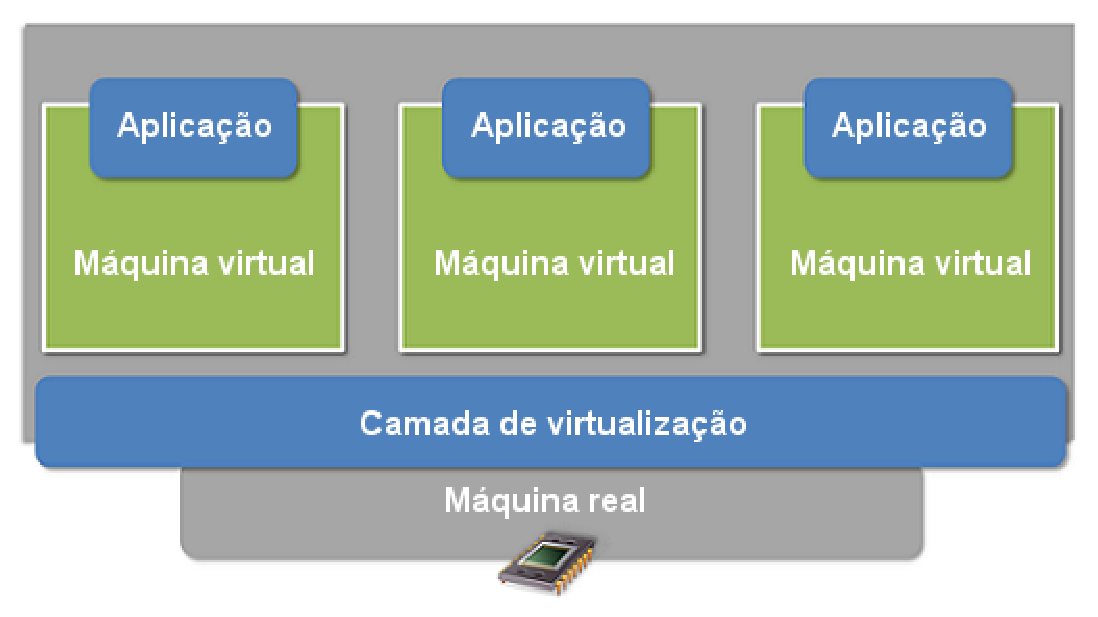
\includegraphics[width=300px]{img/virtcomponentes.eps}
 \caption{Componentes da virtualização.}
 \label{fig:virtcomponentes}
 Fonte: \citet{andrade2011}
\end{figure}

\subsection{Arquiteturas de máquinas virtuais de sistema}
\label{section:virtarquit}

Existem basicamente duas arquiteturas de hipervisor de sistema, que são apresentadas na Figura \ref{fig:vms_arquiteturas} \cite{maziero2013}:

\begin{itemize}
 \item Hipervisores nativos: esse hipervisor executa diretamente sobre o \textit{hardware}, ou seja, sem um sistema operacional
 hospedeiro. Neste caso, o hipervisor nativo faz a multiplexação dos recursos do \textit{hardware} (memória, disco rígido, interface de rede, 
 entre outros) e disponibiliza esses recursos para as máquinas virtuais. Alguns exemplos de sistemas que utilizam essa arquitetura de hipervisor 
 são o \textit{IBM 370} \cite{ibm370}, o \textit{Xen} \cite{xen} e o \textit{VMware ESXi} \cite{vmwareesxi};
 \item Hipervisores convidados: esse tipo de hipervisor executa sobre um sistema operacional hospedeiro e utiliza os recursos desse sistema 
 para gerar recursos para as máquinas virtuais. Normalmente esse tipo de arquitetura suporta apenas um sistema operacional convidado para cada 
 hipervisor. Exemplos de \textit{softwares} que possuem esse tipo de arquitetura são o \textit{VirtualBox} \cite{virtualbox}, 
 o \textit{VMware Player} \cite{vmwareplayer} e o \textit{QEmu} \cite{qemu}.
\end{itemize}

\begin{figure}[h!]
 \centering
 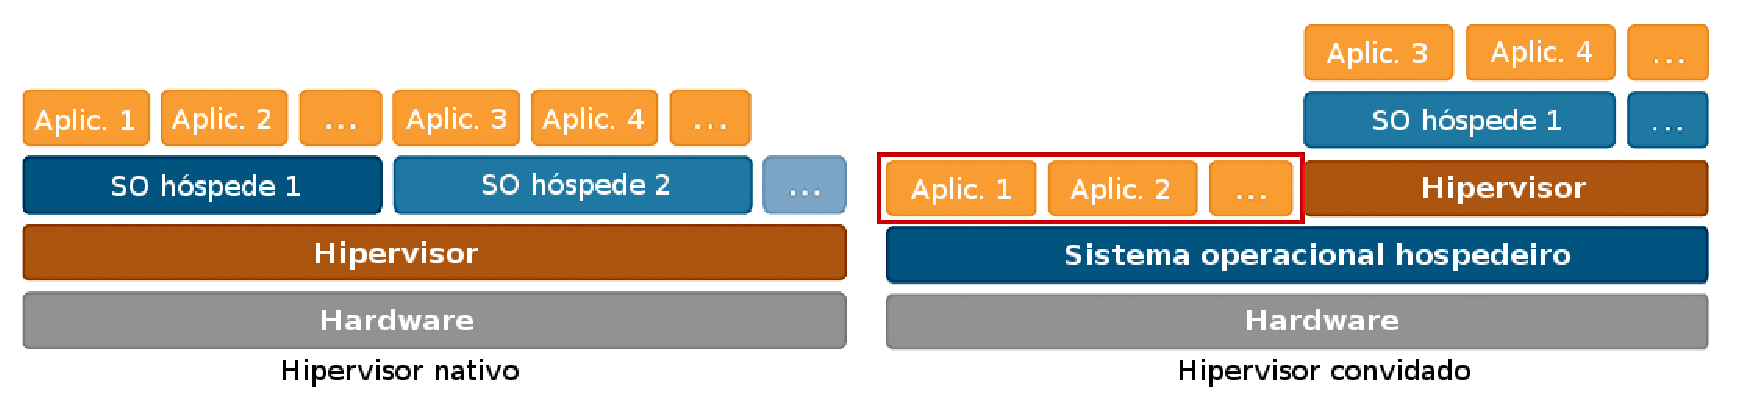
\includegraphics[width=430px]{img/vms_arquiteturas.eps}
 \caption{Arquiteturas de máquinas virtuais de sistema.}
 \label{fig:vms_arquiteturas}
 Fonte: \citet{macedo2016}
\end{figure}

Os hipervisores convidados são mais flexíveis que os nativos, pois podem ser facilmente instalados ou removidos de um sistema operacional já 
instalado. Por outro lado, os hipervisores nativos possuem melhor desempenho pois acessam o \textit{hardware} de forma direta.

%\subsection{Níveis de virtualização}
%\label{section:virtniv}
%\begin{itemize}
% \item Virtualização de recursos: neste tipo de virtualização os recursos como memória e disco, além das instruções 
% privilegiadas (\textit{system \ac{ISA}}) são virtualizadas. Somente a interface \ac{ISA} de usuário é utilizada diretamente, 
% por isso o desempenho do sistema convidado é mais próximo a um sistema executando diretamente sobre um \textit{hardware}. O 
% \textit{VirtualBox} e o \textit{VirtualPC da Microsoft} são exemplos de virtualização de recursos;
% \item Virtualização completa: na virtualização completa todas interfaces são virtualizadas. Sendo assim o hipervisor fornece uma
% interface distinta ao sistema operacional convidado. Esse tipo de virtualização possui um eficiência menor, por outro lado ele
% permite executar sistemas operacionais em plataformas distintas a qual foram projetadas inicialmente. Por exemplo, o 
% \textit{MS Virtual PC for MAC}, que permite executar o sistema \textit{Windows} sobre plataforma de \textit{hardware} \textit{PowerPC}.
%\end{itemize}

%Tendo essas classificações, pode-se combiná-las para se obter quatro maneiras diferentes de implementar virtualização. Na Figura 
%\ref{fig:vms_classificacao} tem-se essas combinações com seus respectivos exemplos.

%\begin{figure}[vms_classificacao]
% \centering
% 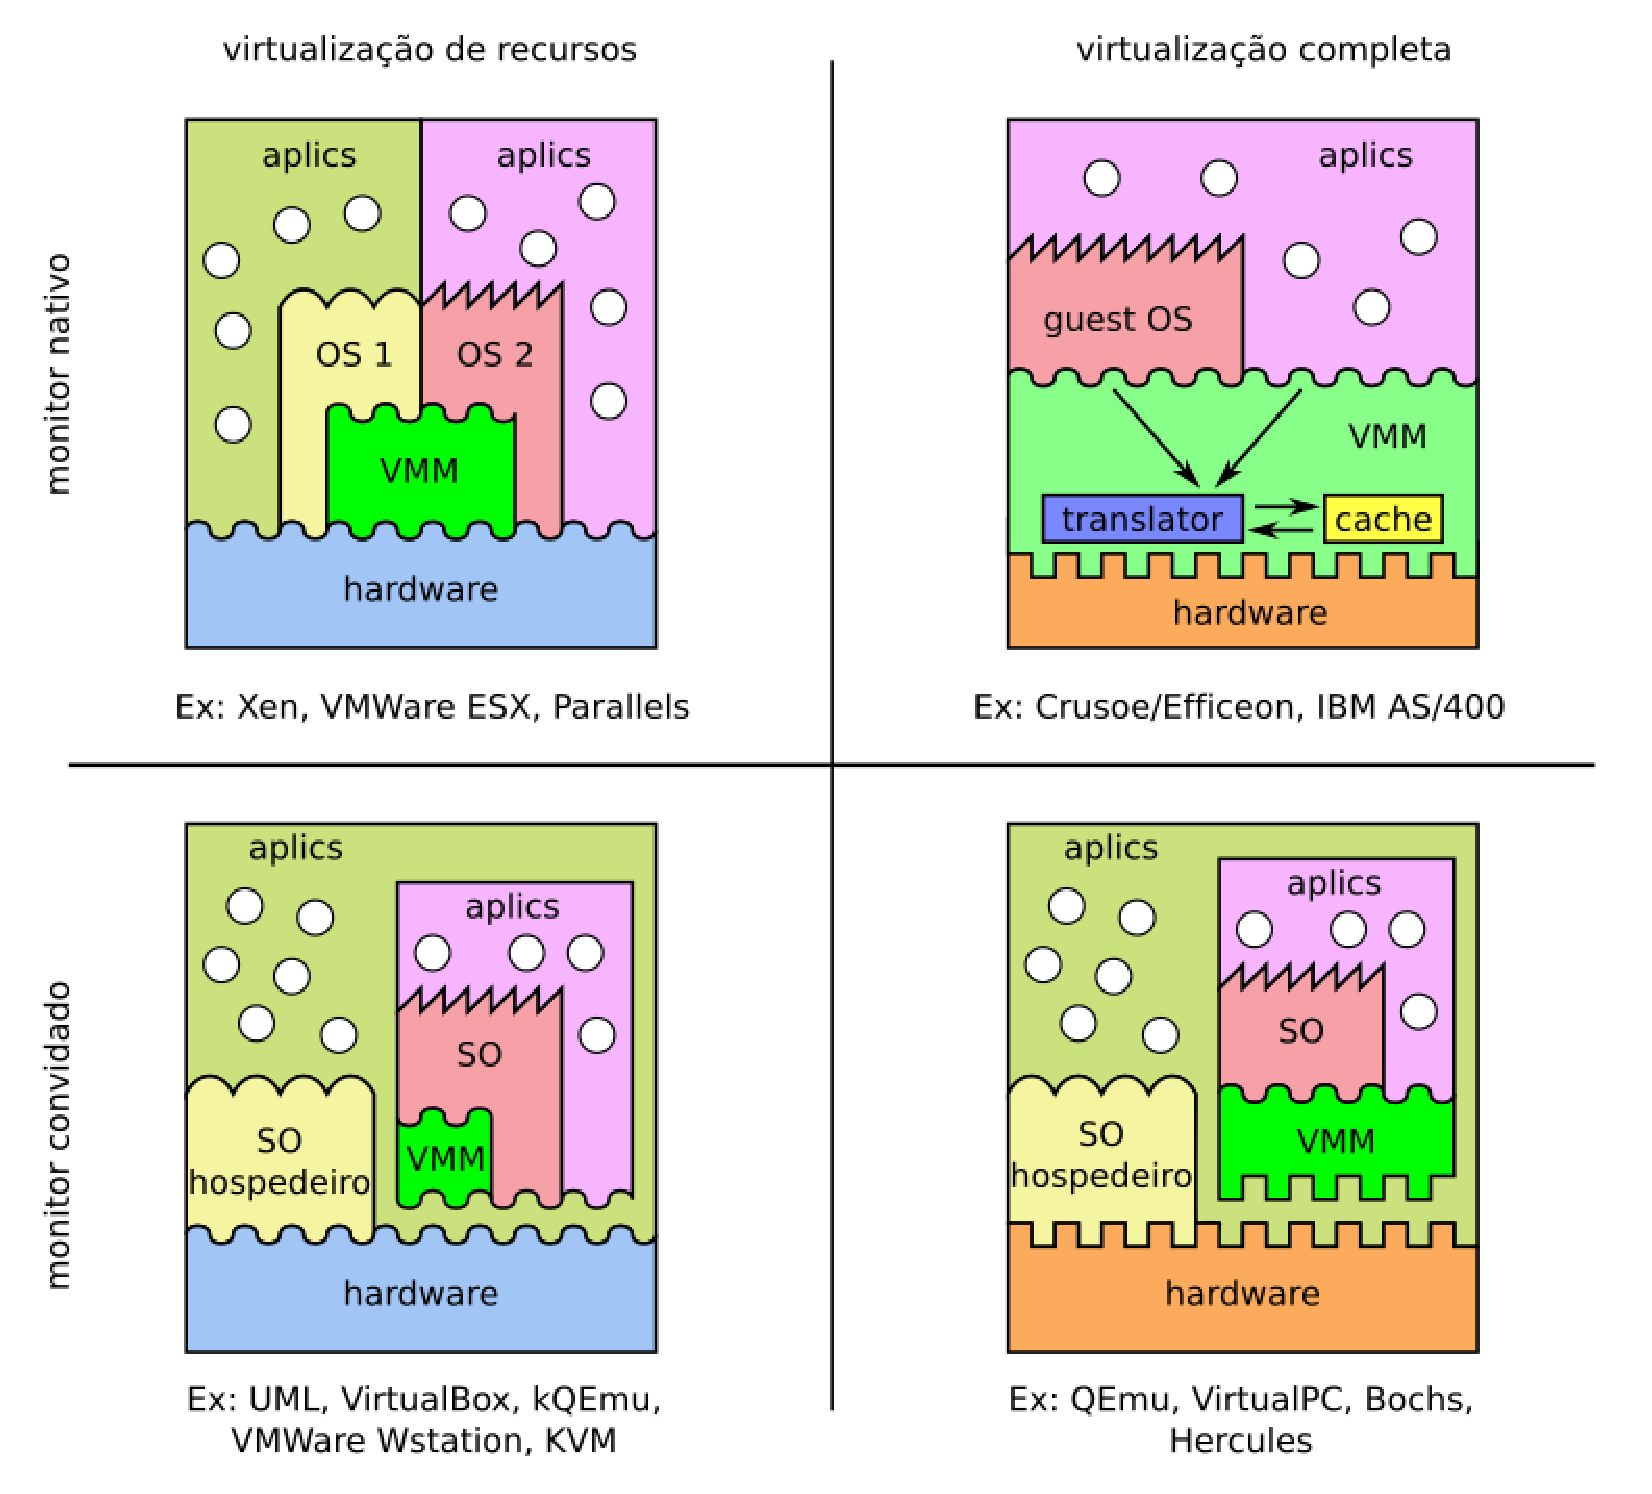
\includegraphics[width=400px]{img/vms_classificacao.eps}
% \caption{Classificação de máquinas virtuais de sistema.}
% \label{fig:vms_classificacao}
% Fonte: \citet{laureano2008}
%\end{figure}

\newpage
\subsection{Implementações de máquinas virtuais de sistema}
\label{section:virtestrat}

As máquinas virtuais de sistema podem ser implementadas usando diferentes estratégias. Atualmente as estratégias mais utilizadas
são a virtualização total e a paravirtualização (Figura \ref{fig:vms_implementacao}):

\begin{figure}[h!]
 \centering
 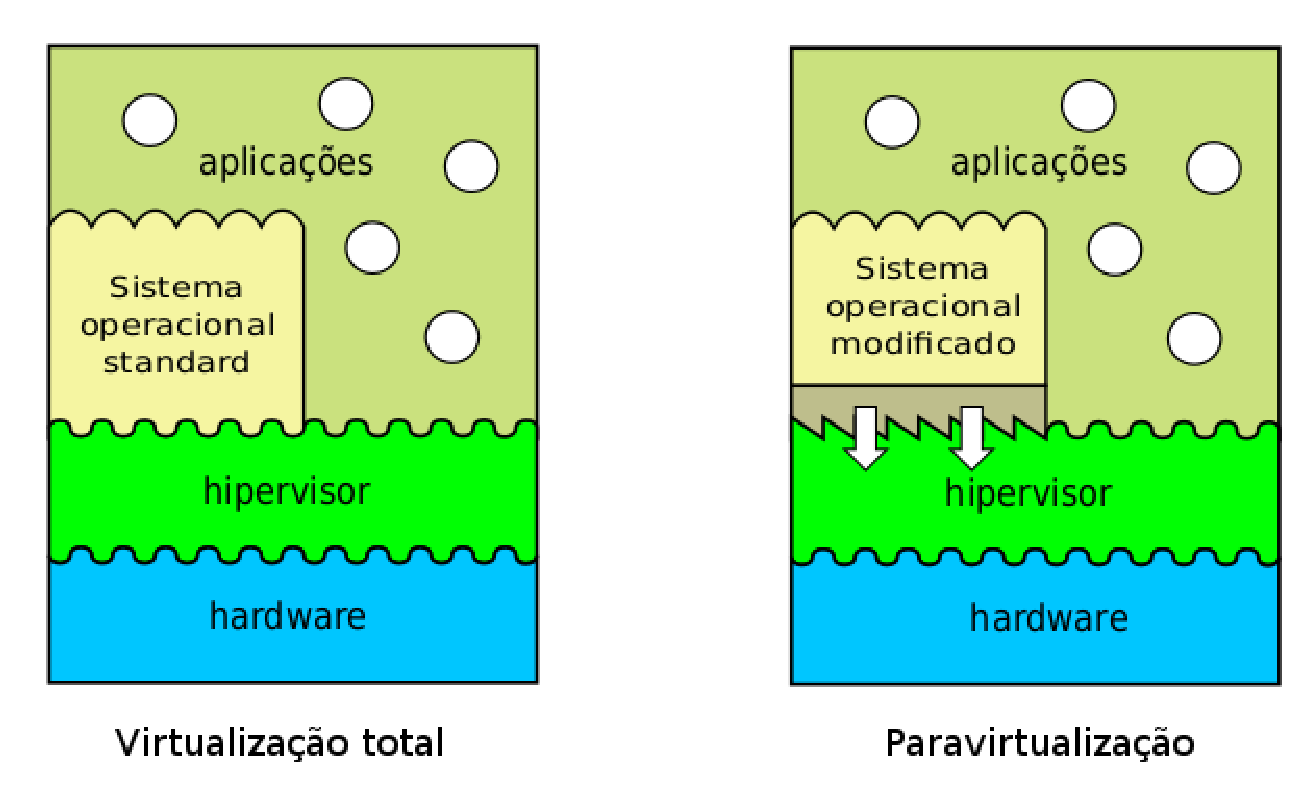
\includegraphics[width=330px]{img/vms_implementacao.eps}
 \caption{Implementações de máquinas virtuais de sistema.}
 \label{fig:vms_implementacao}
 Fonte: \citet{maziero2013}
\end{figure}

\begin{itemize}
 \item Virtualização total: nesta estratégia todas as interfaces de acesso ao \textit{hardware} são virtualizadas. Desta forma, possibilita-se 
 que os sistemas operacionais convidados executem como se estivessem diretamente sobre o \textit{hardware}. Na virtualização total o conjunto de 
 instruções do processador é acessível somente ao hipervisor, sendo que essa estratégia utiliza tradução dinâmica\footnote[1]{A tradução dinâmica 
 analisa e reorganiza as instruções de um sistema convidado para melhorar o desempenho da execução. Além disso, a tradução dinâmica converte as 
 instruções do sistema convidado para o sistema real.} para executar as instruções do sistema convidado. A grande vantagem dessa estratégia é a 
 possibilidade de um sistema convidado ser executado sem a necessidade de ser modificado. Porém, essa estratégia possui um desempenho inferior 
 devido ao fato do hipervisor intermediar todas as chamadas de sistemas e operações do sistema convidado. Um exemplo de ferramenta que utiliza 
 a virtualização total é o \textit{QEmu} \cite{qemu};
 \item Paravirtualização: nesta estratégia a interface entre o hipervisor e o sistema operacional convidado foi modificado para se obter uma 
 maior eficiência. Destaca-se que essa estratégia de implementação utiliza uma arquitetura de hipervisor nativo. 
 As modificações na interface de sistema (\textit{system \ac{ISA}}) exigem que o sistema operacional convidado seja adaptado para o hipervisor, 
 para possibilitar a execução sobre a plataforma virtual. Para essa adaptação, o hipervisor disponibiliza uma \ac{API}, para que os 
 sistemas convidados possam acessar o \ac{ISA} de sistema. Contudo, a interface de usuário é mantida, assim, as aplicações do sistema convidado 
 não precisam ser modificadas \cite{maziero2013}.
\end{itemize}

A paravirtualização possui um desempenho superior se comparada a virtualização total, pois acessa alguns recursos de forma direta, sendo que 
o hipervisor é responsável somente por impedir que o sistema convidado execute operações indevidas. Como exemplo pode-se citar o controle de
acesso à memória feito pelo hipervisor. Na virtualização total o hipervisor reserva um espaço para cada sistema convidado, que por sua vez, 
acessa a memória como se fosse uma memória física, ou seja, inicia o seu endereçamento na posição zero. Sendo assim, cada vez que o sistema 
convidado acessar a memória, o hipervisor precisará converter os endereços do sistema convidado para os endereços reais de memória. Já na 
paravirtualização, o hipervisor informa ao sistema convidado a área de memória que ele poderá utilizar, assim, não sendo necessário nenhuma 
conversão de endereços.

Apesar de apresentar um desempenho inferior, a virtualização total possui uma maior portabilidade, ou seja, permite que sistemas operacionais 
executem como convidados sem a necessidade de serem modificados. Desta forma, qualquer sistema operacional pode ser instalado em um ambiente 
de virtualização total. Além disso, essa técnica permite virtualizar um sistema operacional já instalado apenas copiando o conteúdo de seu disco 
rígido, sem a necessidade de reinstalar esse sistema operacional e reconfigurar todas as aplicações.

\section{Vantagens das máquinas virtuais}
\label{section:virtvantag}

De modo geral, a principal vantagem das máquinas virtuais de aplicação é a possibilidade de executar uma mesma aplicação em diversos sistemas 
operacionais sem a necessidade de recompilar a mesma. Já para máquinas virtuais de sistema, destaca-se a possibilidade de executar mais de um 
sistema operacional sobre um mesmo \textit{hardware}. Nas próximas seções serão descritas as principais utilizações e vantagens da virtualização 
de \textit{desktops} e de servidores.

\subsection{Virtualização de Desktop}
\label{section:virtdesk}

A portabilidade é uma das grandes vantagens da virtualização, que também pode ser aplicada em \textit{desktops}. Pode-se citar como exemplo, 
o desenvolvimento de \textit{software} para diversos sistemas operacionais sem a necessidade de aquisição de um computador físico para a instalação
de cada sistema operacional. Assim, a virtualização de \textit{desktops} pode ser utilizada em ambientes de desenvolvimento, pois possibilitam 
a execução de múltiplas plataformas de desenvolvimento sem comprometer o sistema operacional original \cite{carissimi2008}. Um exemplo é o 
\textit{VMware Workstation}, que possibilita a virtualização em \ac{PC}s para fins de desenvolvimento de \textit{software} \cite{vmware2016}.

Em empresas pode-se ainda utilizar a virtualização de \textit{desktops}, através da configuração de terminais remotos nos computadores e um 
servidor para centralizar as máquinas virtuais. Com isso torna-se mais simples a manutenção dos \textit{desktops}, além disso, estes necessitam 
de um \textit{hardware} de menor valor, uma vez que esses executarão apenas um terminal remoto. Por fim, essa técnica possibilita uma maior 
segurança dos dados, pois os dados serão armazenados em um local seguro, como por exemplo, um \textit{data center}. Exemplos desse tipo de 
virtualização são o \textit{Xen Desktop} \cite{xendesktop} e o \textit{VMware Horizon View} \cite{vmwareview}.
%Em empresas pode-se utilizar virtualização de \textit{desktops} para reduzir a subutilização dos \textit{desktops}, que pode ser feito através da
%colaboração com projetos científicos de \textit{clusters} de computadores virtuais \cite{carissimi2008}. %exemplo seti@home

Para usuários de computadores em geral a virtualização também é interessante, uma vez que esses podem necessitar de um \textit{software} que não
está disponível para a plataforma utilizada. Deste modo, a virtualização possibilita executar diferentes sistemas operacionais no computador do 
usuário. Por exemplo, para um usuário de sistema operacional \textit{MacOS} é comum a necessidade de executar aplicações que não existem para a 
sua plataforma, sendo assim esse pode utilizar uma máquina virtual para executar essas aplicações.

Pode-se também encontrar virtualização de \textit{desktops} em laboratórios de ensino, devido a necessidade de executar diferentes sistemas 
operacionais para determinadas disciplinas. Isso é necessário quando pretende-se configurar e executar aplicações para fim de experimentos ou
aprendizagem, com isso, essas ações não afetarão o sistema hospedeiro. A grande vantagem da utilização de máquinas virtuais nesse tipo de 
ambiente é a facilidade na manutenção, pois as máquinas virtuais podem ser restauradas de forma simples.

\subsection{Virtualização de servidores}
\label{section:virtdesk}

Em muitos casos as empresas utilizam serviços distribuídos entre diferentes servidores físicos, como por exemplo, servidores de \textit{e-mail}, 
hospedagens de sites e banco de dados. Essa estrutura faz com que alguns recursos fiquem ociosos, pois em muitos casos esses serviços necessitam 
de uma quantidade de recursos inferior ao que servidor físico oferece. Por exemplo, um serviço de transmissão de \textit{streaming} de áudio 
utiliza pouco acesso ao disco rígido, porém utiliza um poder de processamento e memória RAM maior. Portanto, uma das grandes vantagens da 
virtualização é um melhor aproveitamento dos recursos. De fato, alocando vários serviços em um único servidor físico tem-se um melhor 
aproveitamento do \textit{hardware} \cite{moreira2006} e, consequentemente, tem-se uma redução nos custos de administração e manutenção 
dos servidores físicos.

% A Figura \ref{fig:virtualizacao_servidores}, o servidor localizado à esquerda, apresenta um servidor tradicional com seu sistema operacional 
% (na cor azul) e suas aplicações (na cor laranja). E o servidor à direita é um servidor de virtualização, que possui o hipervisor 
% (na cor azul claro) e suas máquinas virtuais acima do hipervisor.
% \begin{figure}[h!]
%  \centering
%  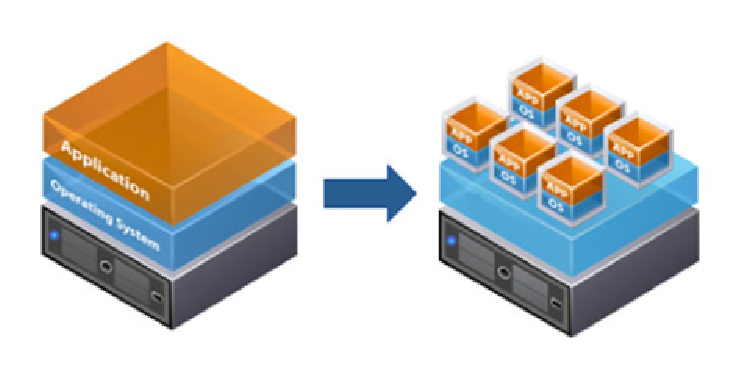
\includegraphics[width=250px]{img/virtualizacao_servidores.eps}
%  \caption{Servidor tradicional e servidor de virtualização.}
%  \label{fig:virtualizacao_servidores}
%  Fonte: \citet{interspire2016}
% \end{figure}

Em um ambiente heterogêneo pode-se também utilizar virtualização, pois ela permite a instalação de diversos sistemas operacionais em um 
único servidor. Esse tipo de virtualização favorece a implementação do conceito ``um servidor por serviço'', que consiste em ter um servidor 
para cada serviço. Além disso, tem-se o isolamento de serviços, ou seja, caso ocorra uma falha de segurança em um serviço, essa falha não 
comprometerá todo o sistema, uma vez que cada serviço estará executando em seu próprio sistema operacional \cite{carissimi2008}.

Outra motivação para a utilização de virtualização em servidores consiste na redução de custos com energia elétrica e equipe. 
Essa redução de custos pode ser obtida através da implantação de servidores mais robustos para substituir dezenas de servidores comuns. 
Além disso, pode-se obter uma redução nos custos com refrigeração, uma vez que essa estrutura proporciona uma redução no número de servidores
e do espaço físico necessário para esses.

Por fim, existe uma técnica chamada \textit{live migration}, ou migração em tempo real. Essa técnica possibilita que uma máquina virtual, 
que está executando em um servidor físico, seja transferida, através da rede, para outro servidor sem ser reiniciada. Nesse processo a máquina 
virtual fica no estado suspenso (por um período curto de tempo) até que o servidor de destino receba os dados necessários para continuar 
a execução da máquina virtual \cite{silva2009}. Essa técnica possibilita a utilização de redundância de \textit{software} e fará parte da 
implementação deste trabalho.

\section{Considerações finais}

Neste capítulo foi apresentado um breve histórico da virtualização e os dois principais grupos de máquinas virtuais existentes que são: máquinas 
virtuais de aplicação e máquinas virtuais de sistema. Também foram apresentadas as vantagens e as estratégias de implementação de máquinas virtuais, 
dando ênfase para as máquinas virtuais de sistema, uma vez que essas serão utilizadas no desenvolvimento deste trabalho. De fato, essas serão 
utilizadas para a implementação da redundância de \textit{software}. No próximo capítulo será feito o levantamento e análise dos serviços 
fornecidos pela empresa que está sendo estudada neste trabalho. Posteriormente, serão apresentados os serviços que são considerados críticos 
e a proposta de solução de alta disponibilidade.

\chapter{Estudo de caso}
\label{cap:estudodecaso}

Este capítulo apresentará a estrutura da empresa que será objetivo de estudo neste trabalho. Esta é uma empresa que fornece serviços de 
hospedagens e também está associada a um provedor de Internet\footnote{É importante salientar que esse provedor utiliza a maior parte dos 
serviços da empresa, pois possui maior número de clientes.}. A empresa possui grande parte de seus clientes localizados na serra do 
Rio Grande do Sul, sendo que atualmente essa empresa possui aproximadamente 9000 clientes. A sede da empresa está localizada na cidade de 
Garibaldi, além disso possui quatro filiais no estado, atendendo aproximadamente xx?? cidades.

A empresa oferece serviços pela internet aos seus clientes, sendo eles: hospedagens de sites, banco de dados, \textit{e-mail}, sistemas de gestão, 
\textit{e-mail marketing}, \textit{backup}, \textit{máquinas virtuais}, autenticação via \ac{ADSL}, rádio \textit{online} e telefonia.
Além disso, o provedor associado fornece aos seus clientes acesso à internet via rádio e acesso à internet por meio de fibra óptica.
A maioria dos serviços são fornecidos por meio de \textit{softwares} de código aberto.

Atualmente a empresa possui redundância de refrigeração e de energia, como pode ser observado na Figura \ref{fig:insteletrica}. 
A redundância de refrigeração é composta por dois ares-condicionados (identificar na figura ??). 
A redundância de energia é feita através de três \textit{nobreaks}, sendo que dois deles (identificar na fig ??) são utilizados para alimentação 
dos servidores e outros equipamentos como por exemplo roteadores, de forma que caso um falhe o outro alimente todos os equipamentos. O terceiro 
\textit{nobreak} (identificar na fig ??) é utilizado para alimentar os computadores dos funcionários de dois setores. 
Além disso, dois geradores (identificar nag fig ??) suprem a necessidade de consumo de energia elétrica do ambiente.
Na imagem também pode-se observar a entrada de energia, com três fases (RGE fase 1, RGE fase 2 e RGE fase 3). Ligado aos \textit{nobreaks} estão 
ligados seis \textit{totens} (são torres que possuem tomadas para plugar os equipamentos). E por fim os \textit{racks} onde ficam os servidores
e o restante dos equipamentos.

\begin{figure}[h!]
 \centering
 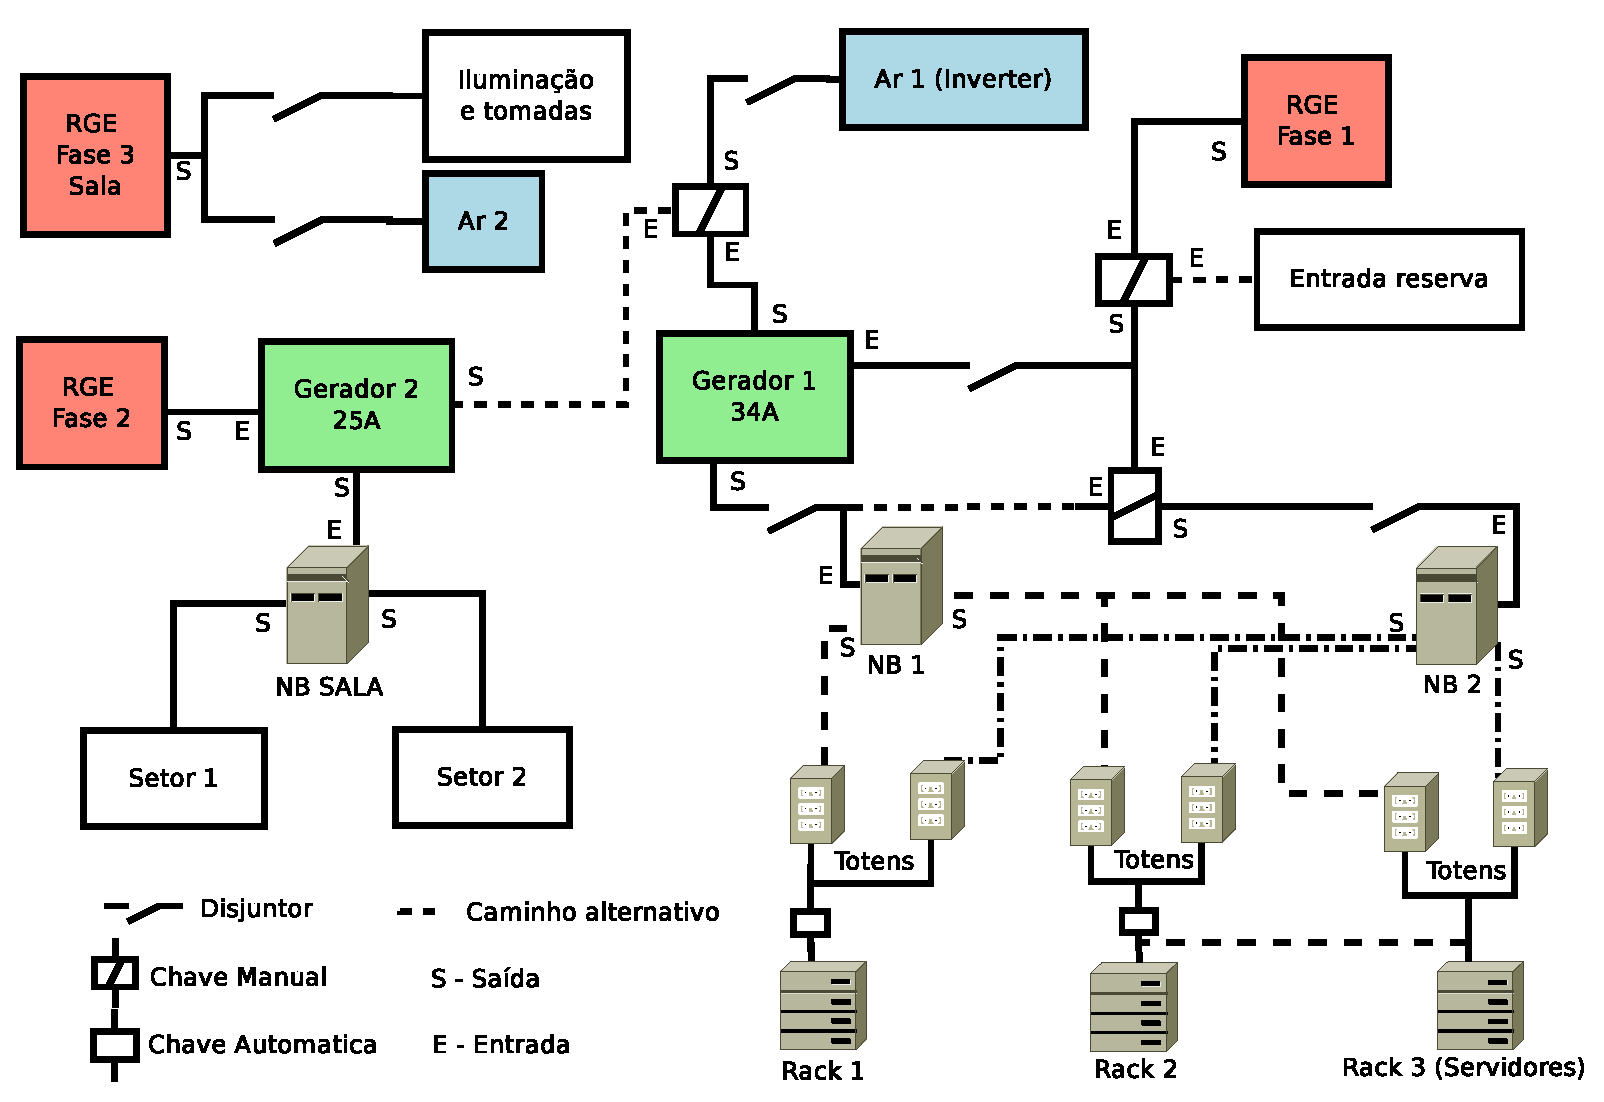
\includegraphics[width=380px]{img/insteletrica.eps}
 \caption{Diagrama de instalação elétrica.}
 \label{fig:insteletrica}
\end{figure}

Nas próximas seções será feita uma descrição da estrutura da empresa. Na Seção \ref{section:ambiente} será descrito o ambiente físico dos 
servidores, com suas estruturas e suas configurações. Na Seção \ref{section:servsemvirt} será descrito os servidores que possuem os seus
serviços instalados diretamente sobre o sistema operacional do servidor, ou seja, sem virtualização.
Na Seção \ref{section:servvirt} será descrito a estrutura de virtualização e todos os serviços fornecidos pelos servidores. 
E na Seção \ref{section:servcrit} será feito a seleção dos serviços críticos através de critérios definidos.

\section{Ambiente físico}
\label{section:ambiente}

A estrutura atual da empresa é composta por quatorze servidores físicos. 
A configuração de \textit{hardware} desses servidores pode ser encontrada na Tabela \ref{tab:servfisicos}, onde tem-se o nome do servidor, 
o modelo, a configuração dos processadores, quantidade de memória, número de discos e a capacidade unitária de cada disco.

\begin{table}[h!]
\caption{Configuração dos servidores físicos.}
\label{tab:servfisicos}
\begin{center}
\def\arraystretch{1}
\setlength{\tabcolsep}{0.15cm}
\begin{tabular}{|l|l|p{5.1cm}|l|p{2.1cm}|}\hline
Servidor & Modelo & Processador & Memória & Disco\\\hline
Bello & & 1 x Intel Core 2 Duo E6750 2.66 GHz & 2 GB DDR2 & 5,5 TB SATA\\\hline
Cacti & Dell PowerEdge 2950 & 2 x Intel Xeon E5310 1.60 GHz & 12 GB DDR2 & 2 x 73 GB SAS\\\hline
Dati & Dell PowerEdge 1850 & 2 x Intel Xeon 3.20 GHz & 4 GB DDR2 & 2 x 146 GB SCSI\\\hline
Monit & & 1 x Intel Core 2 Quad Q9550 2.83 GHz & 4 GB DDR2 & 120 GB SSD\\\hline
Nino & & 1 x Intel Core 2 Duo E4500 2.20 GHz & 4 GB DDR2 & 500 GB SATA\\\hline
Sfrunhon & & 1 x Intel Xeon X3330 2.66 GHz & 8 GB DDR2 & 750 GB SATA\\\hline
Vigilante & & 1 x Intel Pentium Dual E2180 2.00 GHz & 4 GB DDR2 & 2,5 TB SATA\\\hline
Brina & Dell PowerEdge 2950 & 2 x Intel Xeon E5410 2.33 GHz & 24 GB DDR2 & 6 x 300 GB SAS\\\hline
Fulmine & IBM System x3650 M4 & 1 x Intel Xeon E5-2650 2.00 GHz & 32 GB DDR3 & 6 x 2 TB SATA\\\hline
Piova & Dell PowerEdge R410 & 2 x Intel Xeon E5530 2.40 GHz & 32 GB DDR3 & 4 x 500G SATA\\\hline
Raggio & HP ProLiant DL360 G7 & 2 x  Intel Xeon E5630 2.53 GHz & 32 GB DDR3 & 4 x 300 GB SAS\\\hline
Tempesta & Dell PowerEdge R620 & 2 x Intel Xeon E5-2620 2.00 GHz & 32 GB DDR3 & 5 x 1 TB SATA 3 x 1,2 TB SAS\\\hline
Tuono & HP ProLiant DL380 G7 & 2 x Intel Xeon E5649 2.53 GHz & 32 GB DDR3 & 6 x 300 GB SAS 2 x 146 GB SAS\\\hline
Venti & Dell PowerEdge R210 II & 1 x Intel Xeon E3-1220 3.10 GHz & 16 GB DDR3 & 2 x 3 TB SATA\\\hline
\end{tabular}
\end{center}
\end{table}

Todos os servidores estão ligados ao \textit{switch}, que provê aos servidores acesso à internet através de um roteador. Para os servidores 
mais importantes são utilizados dois cabos de rede que estão ligados a um \textit{switch} \textit{gigabit}, assim possibilitando
a configuração de \textit{link aggregation} que permite configurar mais de uma interface de rede física em uma interface agregada, com isso 
pode-se dobrar a capacidade de tráfego de dados. 
O diagrama da Figura \ref{fig:servfisicos} demonstra uma visão geral da estrutura física dos servidores da empresa. 

\begin{figure}[h!]
 \centering
 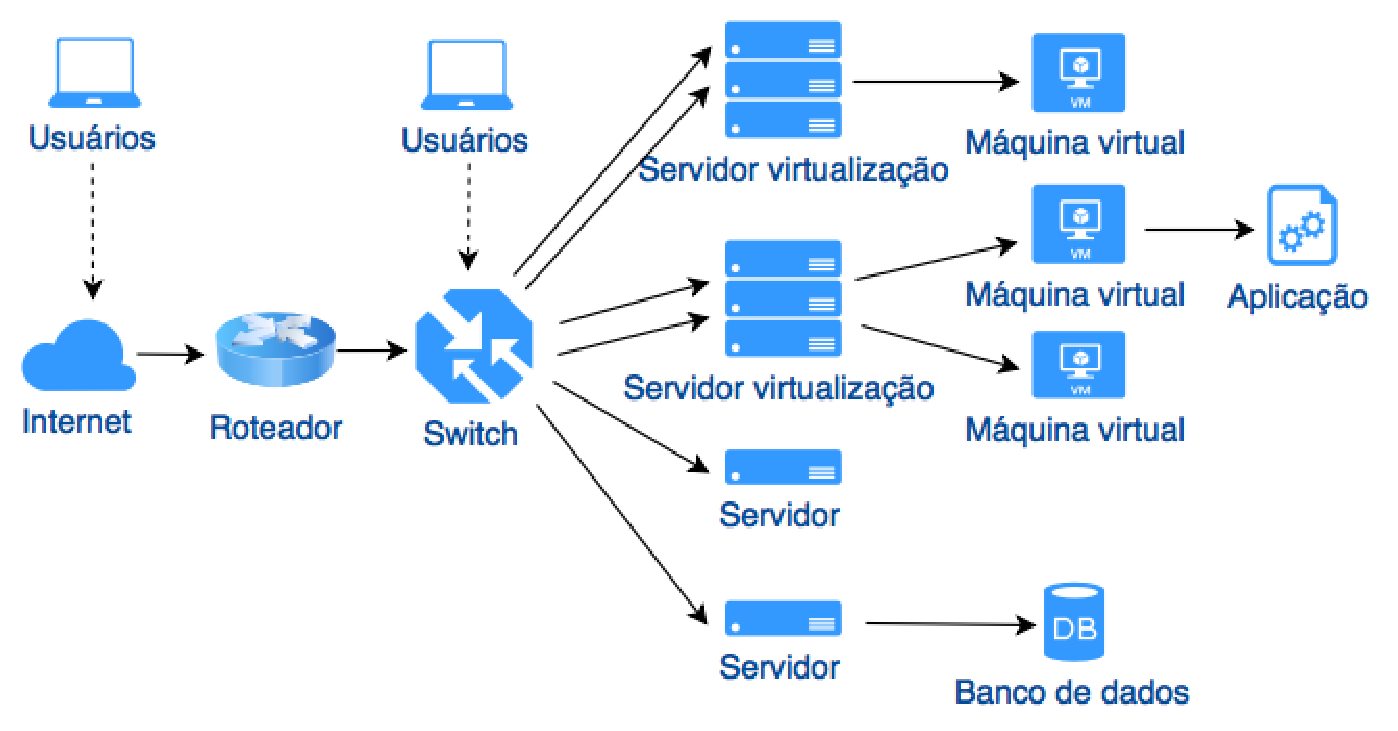
\includegraphics[width=380px]{img/servfisicos.eps}
 \caption{Modelo de estrutura física. BORDA ??}
 \label{fig:servfisicos}
\end{figure}

A Figura \ref{fig:servrack} demonstra, através de uma foto, todos os servidores, inclusive o \textit{switch}, montados em um \textit{rack}.

\begin{figure}[h!]
 \centering
 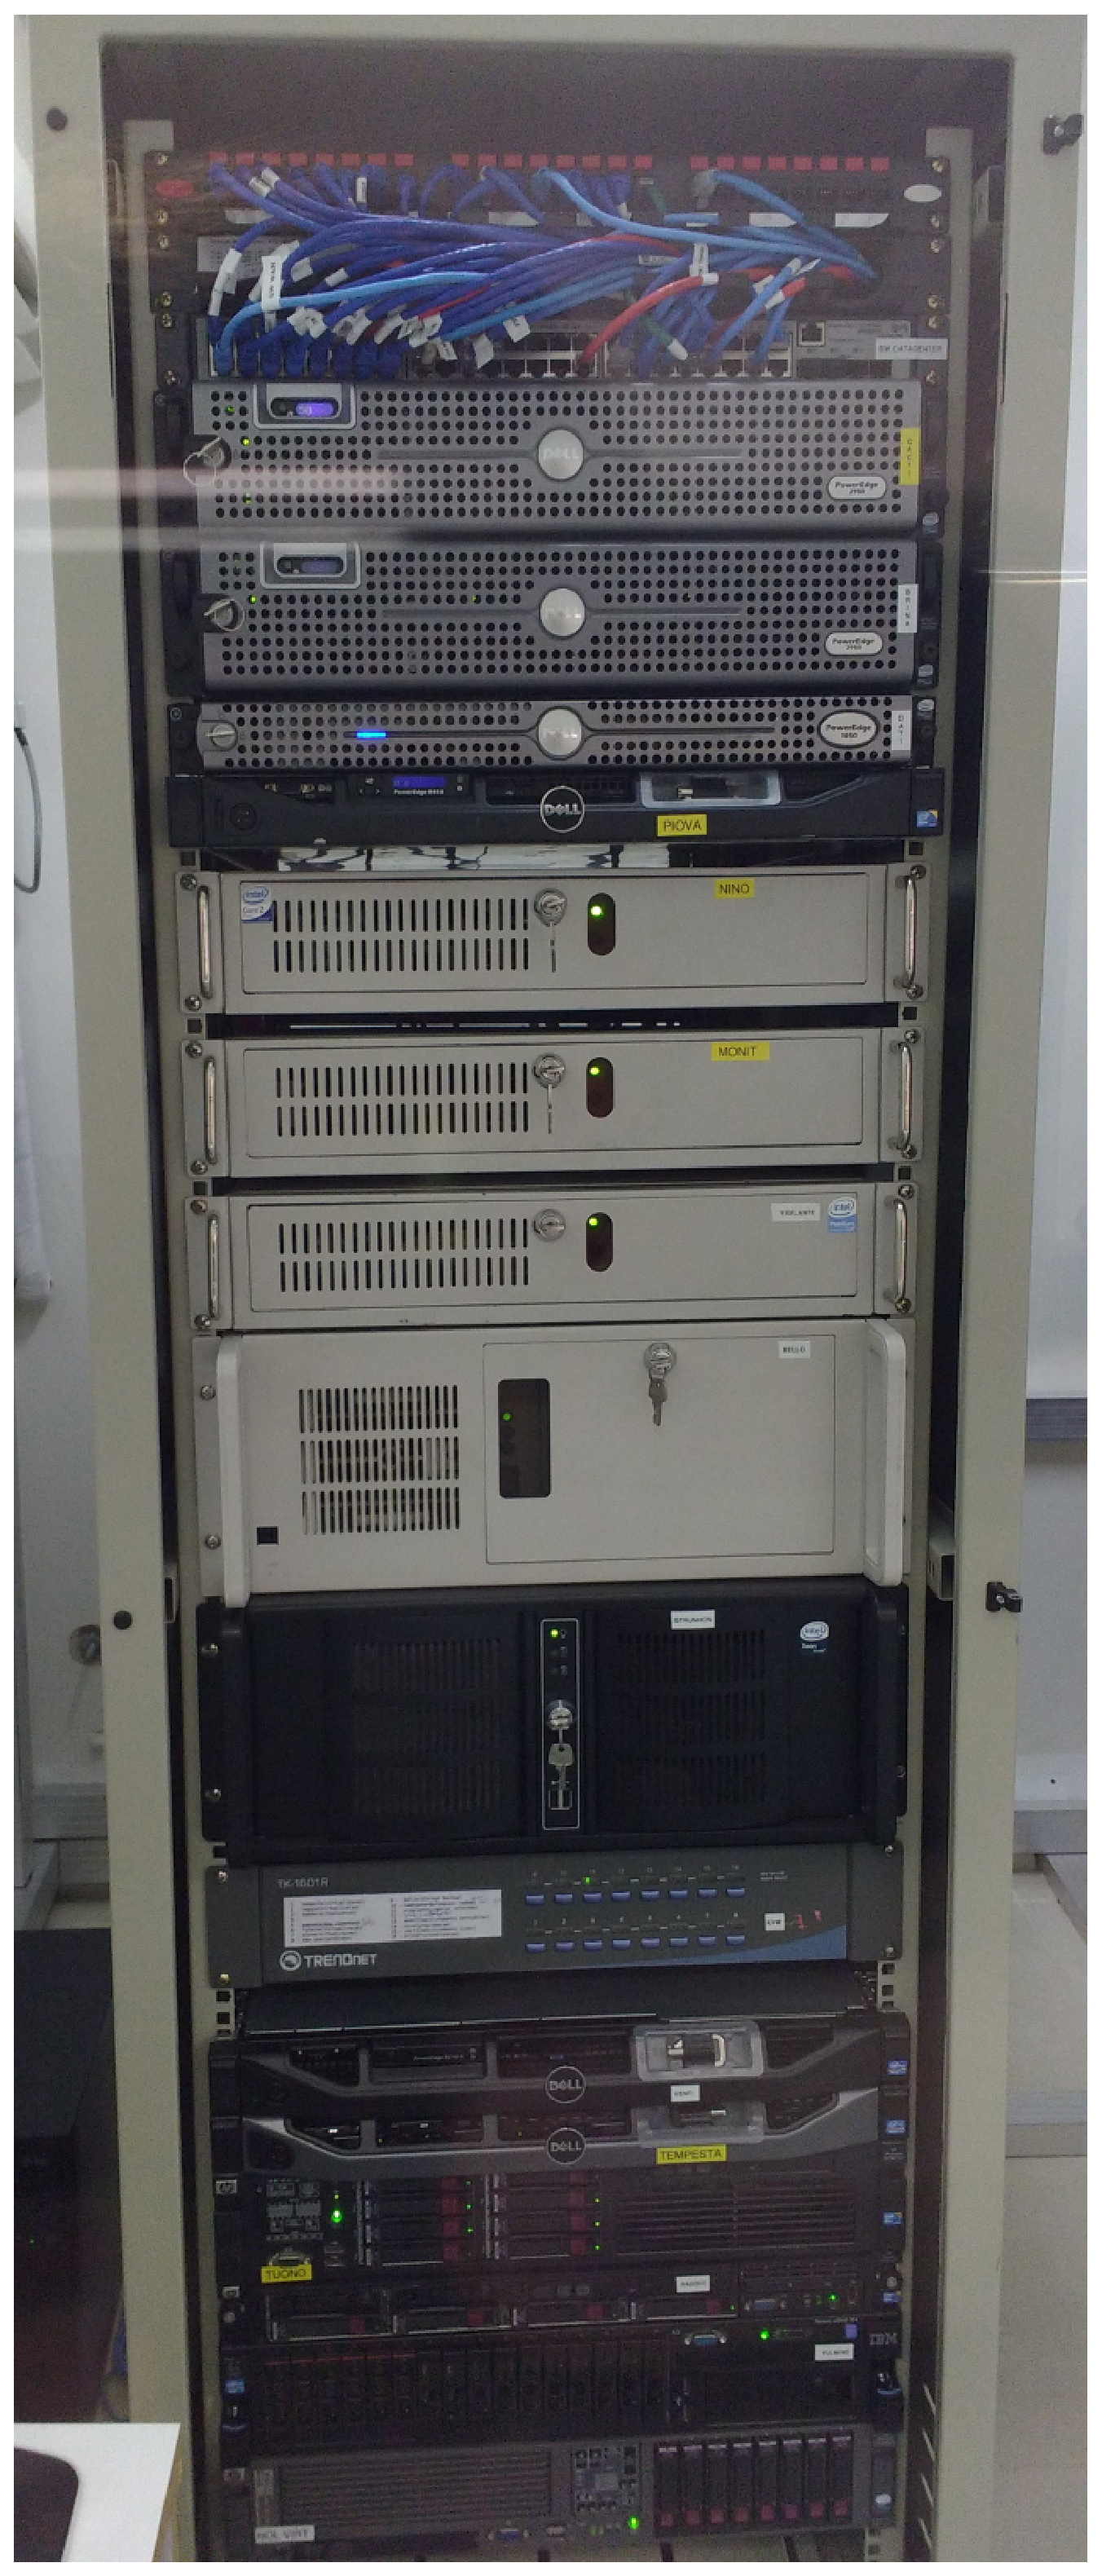
\includegraphics[width=120px]{img/servrack.eps}
 \caption{Imagem do \textit{rack} e dos servidores.}
 \label{fig:servrack}
\end{figure}

\section{Servidores sem virtualização}
\label{section:servsemvirt}

Atualmente existem sete servidores que possuem serviços onde executam sobre o sistema operacional nativo, ou seja, sem virtualização. 
Eles são os sete primeiros servidores da Tabela \ref{tab:servfisicos}, e são listados a seguir:
\begin{itemize}
 \item Bello: esse servidor possui o sistema operacional \textit{Ubuntu 14.04 \ac{LTS}} \cite{ubuntu}. Sua função é armazenar dados de 
 \textit{backup}, para isso ele possui a ferramenta \textit{Bacula Storage 5.2.6} \cite{bacula} instalado, que o possibilita fazer esse 
 armazenamento. Sendo que a ferramenta que é responsável por fazer o \textit{backup} está instalada em um outro servidor que será detalhado na 
 Seção \ref{section:serv_venti};
 
 \item Cacti: um dos servidores de monitoramento da rede do provedor. Esse utiliza a distribuição \textit{CentOS 6.6} \cite{centos} e executa a 
 aplicação \textit{Cacti 0.8.8b} \cite{cacti}, que é uma ferramenta de código aberto desenvolvida para monitorar qualquer equipamento de rede que 
 suporte o protocolo \ac{SNMP}. Ela monitora atualmente a maior parte da rede \textit{core} e a rede \textit{backbone} tanto dos clientes de 
 internet via rádio, como de fibra óptica;
 
 \item Dati: é o servidor de banco de dados principal. Esse possui o sistema operacional \textit{Ubuntu 14.04 \ac{LTS}} \cite{ubuntu}. 
 O serviço que executa sobre esse servidor é um sistema gerenciador de banco de dados \textit{MySQL 5.5.49} \cite{mysql}, que armazena os dados 
 das aplicações de \textit{ZoneMinder} \cite{zoneminder} (servidor de câmeras) e \textit{Icewarp Server} (servidor de \textit{e-mail}), que serão 
 detalhados posteriormente;
 
 \item Monit: esse servidor faz o monitoramento dos demais servidores. Ele possui o sistema operacional \textit{Ubuntu 12.04 \ac{LTS}} 
 \cite{ubuntu}, executando as aplicações \textit{Nagios 3.2.3} \cite{nagios} e \textit{Munin 1.4.6} \cite{munin}, ambos \textit{softwares} livres. 
 O \textit{Nagios} monitora o \textit{hardware} e os serviços que estão executando em cada servidor. Para alguns serviços é utilizado um cliente 
 \textit{Nagios}. O segundo, \textit{Munin}, é responsável por gerar gráficos de monitoramento. Com ele pode-se criar, por exemplo, gráficos 
 com a utilização: do processador, memória, disco, temperatura e velocidade dos \textit{fans};
 
 \item Nino: esse é o servidor utilizado pelo setor de desenvolvimento de \textit{software}. Suas aplicações executam sobre o sistema operacional 
 \textit{Ubuntu 14.04 \ac{LTS}} \cite{ubuntu}, sendo que serviços fornecidos pelo servidor são servidor \textit{web} (\textit{Apache 2.4.7} 
 \cite{apache} e \textit{\ac{PHP} 5.5.9} \cite{php}), sistema gerenciador de banco de dados (\textit{MySQL 5.5.49} \cite{mysql} e 
 \textit{PostgreSQL 9.3.13} \cite{postgres}), compartilhamento de arquivos (\textit{Samba 4.3.9} \cite{samba}), controle de versões de 
 \textit{software} (\textit{\ac{SVN} 1.8.8} \cite{svn}), gerenciador de \textit{bugs} (\textit{Trac 1.0.1} \cite{trac}) e mensagens instantâneas 
 (\textit{Ejabberd 2.1.11} \cite{ejabberd});
 
 \item Sfrunhon: outro servidor de monitoramento da rede do provedor. Esse utiliza a distribuição \textit{CentOS 6.3} \cite{centos} e executa a 
 aplicação \textit{Cacti 0.8.8a} \cite{cacti}. Esse servidor monitora atualmente o tráfego dos clientes, tanto de internet via rádio, como de 
 fibra óptica;
 
 \item Vigilante: esse servidor é responsável por capturar e armazenar \textit{streaming} de vídeo das câmeras do provedor. Ele possui o sistema 
 operacional \textit{Ubuntu 14.04 \ac{LTS}} \cite{ubuntu}, e executa a aplicação \textit{ZoneMinder 1.29} \cite{zoneminder}, que é o 
 \textit{software} responsável pela captura e armazenamento das as imagens das câmeras do provedor.
\end{itemize}

\section{Servidores com virtualização}
\label{section:servvirt}

Os servidores de virtualização possuem suas respectivas \ac{VM}s, que executam aplicações. Para virtualização utiliza-se o hipervisor 
\ac{KVM} e a ferramenta \textit{QEmu}, sendo que ambos são projetos de \textit{software} livre. Procurou-se manter um ambiente homogêneo 
com o objetivo de facilitar a manutenção, para isso utilizou-se o mesmo hipervisor e o mesmo sistema operacional para os servidores hospedeiros. 
Esse sistema operacional é o sistema de código aberto \textit{Ubuntu 14.04 \ac{LTS}} \cite{ubuntu}.
Além disso, esses servidores possuem redundância de \textit{hardware}, com fonte de alimentação e discos configurados através de um \ac{RAID}. 
Em seridores com mais de dois discos geralmente é utilizado \ac{RAID} 5. Já em servidores que possuem apenas dois discos é utilizado \ac{RAID} 1 
(espelhamento de discos). O ambiente também possui uma redundância do cabeamento, como visto anteriormente.

A empresa fornece serviços diversos, desde hospedagens de sites até \ac{DNS} recursivo para o provedor de internet. Atualmente sete servidores 
são utilizados para virtualizar sistemas, que são os últimos sete servidores da Tabela \ref{tab:servfisicos}, sendo que existem quarenta e seis 
\ac{VM}s distribuídas entre os sete servidores de virtualização. Nas próximas seções serão descritos esses servidores, suas respectivas 
máquinas virtuais e serviços.

\subsection{Servidor Brina}
\label{section:serv_brina}

O servidor Brina possui duas \ac{VM}s como pode ser visto na Figura \ref{fig:servidor_brina} juntamente com seus respectivos serviços. 
Esses serviços são listados a seguir:
\begin{itemize}
 \item \textit{Masterauth}: sua configuração é 1 \textit{core} para processamento, 1,5 GB de memória e 8 GB de disco. O sistema operacional é o 
 \textit{Ubuntu 14.04 \ac{LTS}} \cite{ubuntu}, sendo que esse servidor fornece o mesmo serviço do servidor \textit{Speedauth} 
 (Seção \ref{section:serv_tuono}), porém para apenas uma parte dos clientes;
 
 \item \textit{Monete}: sua configuração é 1 \textit{core} de processamento, 3 GB de memória e 50 GB de disco. Esse servidor possui o 
 sistema operacional \textit{Ubuntu 14.04 \ac{LTS}} \cite{ubuntu}, sendo um servidor \textit{web} dedicado para o site do provedor, com 
 configurações personalizadas. Para isso ele utiliza os \textit{softwares} \textit{Apache 2.4.7} \cite{apache}, \textit{\ac{PHP} 5.5.9} \cite{php} 
 (com \textit{PHP-FPM 5.59}) e \textit{MySQL 5.5.49} \cite{mysql}.
\end{itemize}

\begin{figure}[h!]
 \centering
 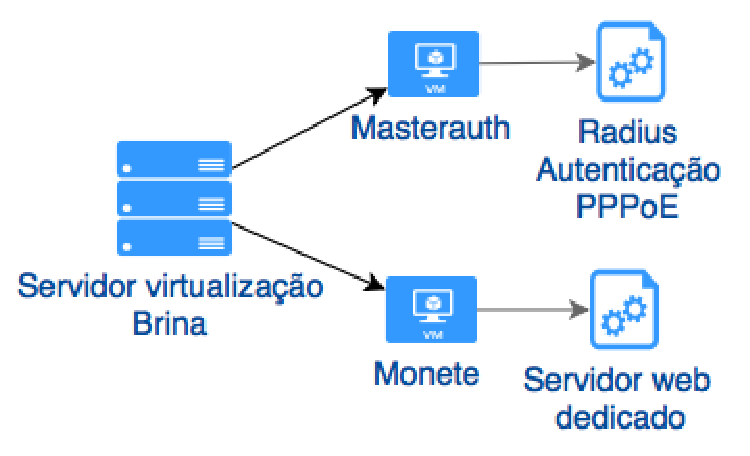
\includegraphics[width=200px]{img/servidor_brina.eps}
 \caption{Servidor de virtualização Brina.}
 \label{fig:servidor_brina}
\end{figure}

\subsection{Servidor Fulmine}
\label{section:serv_fulmine}

O servidor Fulmine possui dez \ac{VM}s como pode ser visto na Figura \ref{fig:servidor_fulmine} juntamente com seus respectivos serviços. 
Esses serviços são listados a seguir:
\begin{itemize}
 \item \textit{Hotspot}: sua configuração é 1 \textit{core} para processamento, 1,5 GB de memória e 8 GB de disco. Esse servidor possui o 
 sistema operacional \textit{Ubuntu 14.04 \ac{LTS}} \cite{ubuntu}, sendo que esse é o servidor de gerência de equipamentos da \textit{Ubiquiti} 
 que fazem \textit{hotspot}, que é uma maneira de disponibilizar a tecnologia \textit{Wi-fi} para prover acesso à internet em ambientes públicos, 
 sendo utilizado pelo provedor;
 
 \item \textit{IPv6Dns}, \textit{IPv6Dns64} e \textit{IPv6Nat64}: suas configurações são 1 \textit{core} para processamento, 1 GB de memória e 
 8 GB de disco. O sistema operacional é o \textit{Ubuntu 14.04 \ac{LTS}} \cite{ubuntu}, sendo que esses servidores fornecem o serviço de \ac{DNS} 
 e \ac{NAT} para navegação \ac{IPv6} do provedor;
 
 \item \textit{Ottico}: esse servidor possui 2 \textit{cores} para processamento, 4 GB de memória e 50 GB de disco. O servidor possui o sistema 
 operacional \textit{Windows 2007 Server Standard} e possui o serviço de \textit{terminal service} para suporte e gerência de fibra óptica do 
 provedor;
 
 \item \ac{PRTG}: esse servidor possui 2 \textit{cores} para processamento, 4 GB de memória e 100 GB de disco. O servidor possui o sistema 
 operacional \textit{Windows 2008 Server R2} e sua função é fazer o monitoramento de tráfego e equipamentos da rede \textit{core} do provedor;
 
 \item \textit{Passata}: esse servidor possui 2 \textit{cores} para processamento, 3 GB de memória e 20 GB de disco. O servidor possui o 
 sistema operacional \textit{Ubuntu 14.04 \ac{LTS}} \cite{ubuntu} e fornece o serviço de \ac{DNS} recursivo, através do \textit{software} 
 \textit{Bind 9.9.5} \cite{bind}. Esse é o servidor primário de \ac{DNS}, sendo o mais importante para navegação dos clientes de todo o provedor;
 
 \item \textit{Roncon}: esse servidor possui 4 \textit{cores} para processamento, 6 GB de memória e 400 GB de disco. Ele possui o sistema
 operacional \textit{Red Hat 5.11} \cite{redhat} e provê acesso a sites \textit{web} desenvolvidos com a linguagem \ac{PHP}. Nele está instalado 
 o \textit{software} \ac{WHM} \cite{whm}, que faz a gerência dos serviços de hospedagens de sites e banco de dados. Além disso, encontra-se 
 disponível a ferramenta \textit{cPanel}, que faz parte do \ac{WHM} e que fornece a gerência de cada hospedagem de site para seu respectivo 
 desenvolvedor. Para fornecer essa hospedagem os seguintes \textit{softwares} estão instalados e configurados: \textit{Apache 2.2.26} \cite{apache}, 
 \textit{\ac{PHP} 5.3.27} \cite{php}, \textit{MySQL 5.1.73} \cite{mysql} e \textit{PostgreSQL 8.4.20} \cite{postgres}.
 Além da hospedagem, esse servidor fornece o serviço de autenticação \ac{ADSL} de terceiros utilizando o \textit{software} \textit{Radius} 
 (\textit{Freeradius 1.1.3} \cite{freeradius});
 
 \item \textit{Servo}: sua configuração é 1 \textit{core} para processamento, 2 GB de memória e 30 GB de disco. Esse servidor possui o 
 sistema operacional \textit{CentOS 6.8} \cite{centos}, sendo que esse servidor fornece, através do \textit{software} \textit{Bind 9.8.2} 
 \cite{bind}, o serviço de \ac{DNS} autoritativo e é o servidor \ac{DNS} secundário dos domínios hospedados pela empresa;
 
 \item \textit{SimplesIP}: esse servidor possui 2 \textit{cores} para processamento, 3 GB de memória e 80 GB de disco. O servidor possui 
 o sistema operacional \textit{CentOS 6.6} \cite{centos} e é o servidor de telefonia do provedor. Esse utiliza como base o \textit{software} 
 livre \textit{Asterisk 1.8.32} \cite{asterisk}.
\end{itemize}

\begin{figure}[h!]
 \centering
 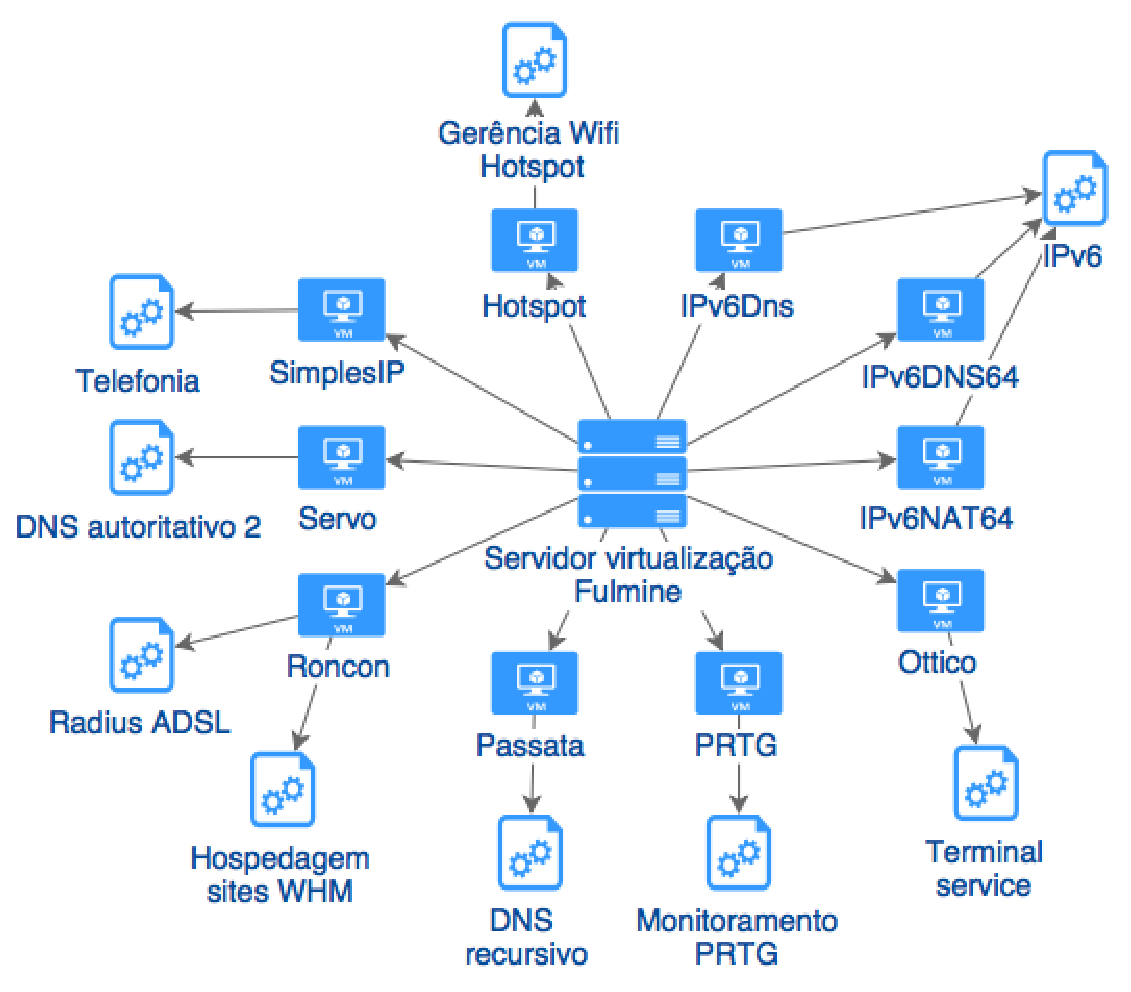
\includegraphics[width=330px]{img/servidor_fulmine.eps}
 \caption{Servidor de virtualização Fulmine.}
 \label{fig:servidor_fulmine}
\end{figure}

\subsection{Servidor Piova}
\label{section:serv_piova}

O servidor Piova possui nove \ac{VM}s como pode ser visto na Figura \ref{fig:servidor_piova} juntamente com seus respectivos serviços. 
Esses serviços são listados a seguir:
\begin{itemize}
 \item \textit{ASP}: esse servidor possui 1 \textit{core} para processamento, 1 GB de memória e 50 GB de disco. O servidor possui o sistema 
 operacional \textit{Windows 2008 Server R2} e provê acesso a sites \textit{web} desenvolvidos com a linguagem \ac{ASP} \cite{asp}, através do
 \textit{software} \textit{\ac{IIS} 7.5} \cite{iis}. Esse servidor possui aproximadamente dez sites hospedados;
 
 \item \textit{CactiBackbone}: esse servidor possui 1 \textit{core} para processamento, 1 GB de memória e 20 GB de disco. Ele é um servidor
 de monitoramento da rede do provedor. Esse utiliza a distribuição \textit{CentOS 6.3} \cite{centos} e executa a aplicação \textit{Cacti 0.8.8a}
 \cite{cacti}. Essa aplicação monitora atualmente uma parte da rede \textit{backbone} do provedor;
 
 \item \textit{Dio}: esse servidor possui 1 \textit{core} para processamento, 1 GB de memória e 17,8 GB de disco. O servidor possui o sistema 
 operacional \textit{Ubuntu 6.06 \ac{LTS}} \cite{ubuntu} e fornece serviço de hospedagens de sites desenvolvidos com a linguagem \ac{PHP} 
 versão 4.4.2. Esses sites são mantidos em um servidor separado devido a incompatibilidade com a versão 5. Esse servidor armazena 
 aproximadamente 10 sites;
 
 \item \textit{FateFurbo}: sua configuração é 2 \textit{cores} para processamento, 4 GB de memória e 80 GB de disco. O sistema operacional é o 
 \textit{Ubuntu 14.04 \ac{LTS}} \cite{ubuntu} e possui um \textit{software} proprietário da empresa \textit{Padtec}, e que faz a gerência de uma 
 parte pequena da fibra óptica do provedor;
 
 \item \textit{FiberHome}: sua configuração é 2 \textit{cores} para processamento, 2 GB de memória e 60 GB de disco. Esse servidor possui o sistema 
 operacional \textit{Windows XP} e possui o \textit{software} \textit{ANM 2000} instalado, para fazer a gerência da fibra óptica do provedor;
 
 \item \textit{Parla}: sua configuração é 1 \textit{core} de processamento, 1 GB de memória e 8 GB de disco. Ele possui o sistema
 operacional \textit{Ubuntu 14.04 \ac{LTS}} \cite{ubuntu} e provê um serviço de mensagens instantâneas, baseado no protocolo \ac{XMPP}. Esse 
 serviço é utilizado para comunicação entre funcionários da empresa e do provedor. O \textit{software} utilizado é o \textit{Ejabberd 2.1.11}
 \cite{ejabberd}, que também é um \textit{software} livre;

 \item \textit{Passata2}: esse servidor possui 1 \textit{core} para processamento, 2 GB de memória e 20 GB de disco. Esse servidor possui o 
 sistema operacional \textit{Ubuntu 14.04 \ac{LTS}} \cite{ubuntu} e fornece o serviço de \ac{DNS} recursivo, através do \textit{software} 
 \textit{Bind 9.9.5} \cite{bind}. Esse é o servidor secundário de \ac{DNS} do provedor;
 
 \item \textit{Postfix}: sua configuração é 1 \textit{core} para processamento, 768 MB de memória e 50 GB de disco. Esse servidor possui o 
 sistema operacional \textit{Ubuntu 14.04 \ac{LTS}} \cite{ubuntu} e é responsável pelo envio de \textit{e-mails}, através do \textit{software} 
 \textit{Postfix 2.11} \cite{postfix}. Os \textit{e-mails} enviados por esse servidor são gerados por uma ferramenta de \textit{e-mail marketing}, que foi
 desenvolvida pela empresa. Esse servidor faz o envio de \textit{e-mails} em massa para divulgação de informações ou produtos;
 
 \item \textit{Servo6}: sua configuração é 1 \textit{core} para processamento, 1,5 GB de memória e 30 GB de disco. Esse servidor possui o 
 sistema operacional \textit{CentOS 6.8} e fornece, através do \textit{software} \textit{Bind 9.8.2} \cite{bind}, o serviço de \ac{DNS} 
 autoritativo, sendo o servidor de \ac{DNS} terciário dos domínios hospedados pela empresa.
\end{itemize}

\begin{figure}[h!]
 \centering
 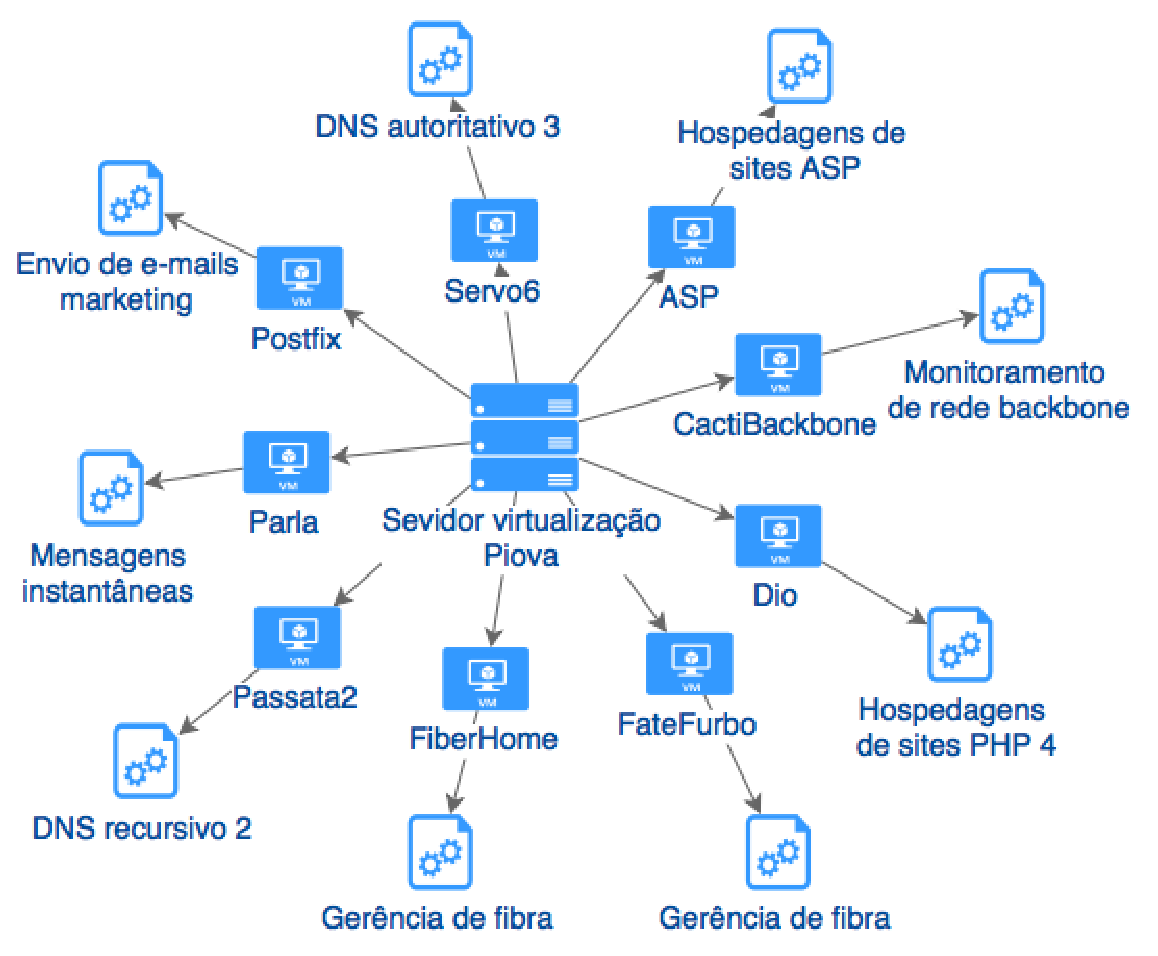
\includegraphics[width=350px]{img/servidor_piova.eps}
 \caption{Servidor de virtualização Piova.}
 \label{fig:servidor_piova}
\end{figure}

\subsection{Servidor Raggio}
\label{section:serv_raggio}

O servidor chamado Raggio executa doze \ac{VM}s (Figura \ref{fig:servidor_raggio}), que fornecem os serviços de virtualização para algumas empresas,
sendo que as máquinas virtuais são instaladas com o sistema operacional da preferência do cliente, e são disponibilizadas através de um serviço 
de acesso remoto, como por exemplo, através de \ac{SSH}.

\begin{figure}[h!]
 \centering
 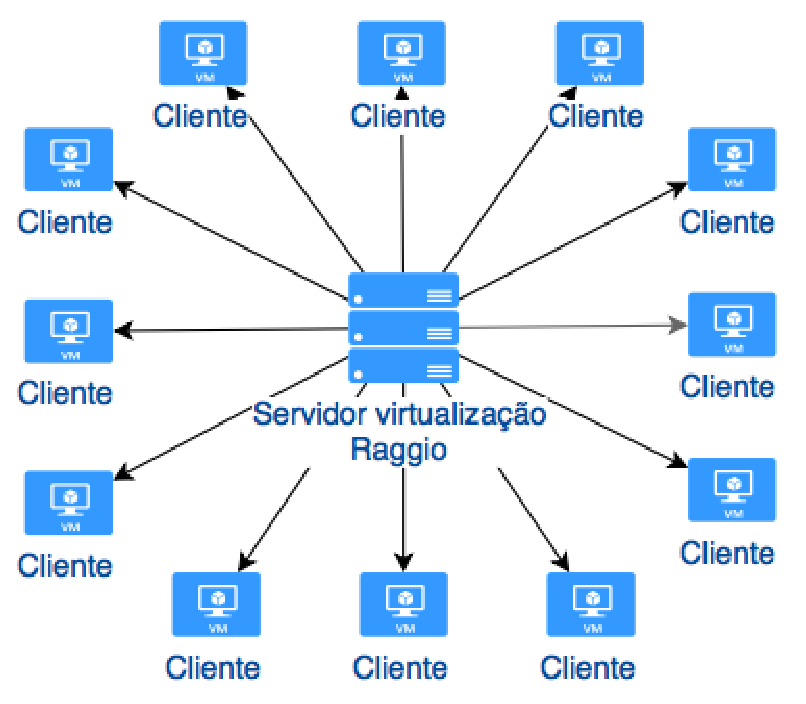
\includegraphics[width=250px]{img/servidor_raggio.eps}
 \caption{Servidor de virtualização Raggio.}
 \label{fig:servidor_raggio}
\end{figure}

\subsection{Servidor Tempesta}
\label{section:serv_tempesta}

O servidor Tempesta possui quatro \ac{VM}s como pode ser visto na Figura \ref{fig:servidor_tempesta} juntamente com seus respectivos serviços. 
Esses serviços são listados a seguir:
\begin{itemize}
 \item \textit{Ledriovardar}: esse servidor possui 2 \textit{cores} para processamento, 2 GB de memória e 80 GB de disco. O servidor possui 
 o sistema operacional \textit{Windows 2008 Server R2} e possui o serviço de \textit{terminal service} para suporte e gerência de fibra 
 óptica do provedor;
 
 \item \textit{Merak}: esse servidor fornece serviço de \textit{e-mail}. Ele possui uma configuração de 6 \textit{cores} para processamento, 
 10 GB de memória e 1000 GB de disco. O servidor possui o sistema operacional \textit{Windows 2008 Server R2} e executa o \textit{software} 
 \textit{Icewarp Server 10.4.4} \cite{icewarp}. Essa aplicação fornece os serviços de envios de \textit{e-mails} (\ac{SMTP}), recebimentos 
 de \textit{e-mails} (\ac{POP} e \ac{IMAP}), Webmail (\ac{PHP}) e Anti-spam;
 %Possui ?? contas sendo que possui uma média de ?? usuários simultâneos...
 %Grande parte das contas estão ociosas pois são oferecidas juntamente com a internet vendida pelo provedor.

 \item \textit{Quebei}: sua configuração é 1 \textit{core} de processamento, 3 GB de memória e 140 GB de disco. Esse servidor possui o 
 sistema operacional \textit{Ubuntu 14.04 \ac{LTS}} \cite{ubuntu} e sua função é gerenciar o \textit{backup} dos outros servidores. Para isso 
 ele utiliza a ferramenta \textit{Bacula 5.2.6} \cite{bacula} (pacote \textit{bacula-director-common 5.2.6}). Além disso, esse servidor possui 
 o sistema gerenciador de banco de dados \textit{MySQL 5.5.49} \cite{mysql} instalado, que esta configurado como \textit{master-slave}, sendo 
 que esse servidor é o \textit{slave} e o servidor \textit{Dati} (Seção \ref{section:servvirt}) é o \textit{master};
 
 \item \textit{Rauco}: esse servidor possui 2 \textit{cores} para processamento, 6 GB de memória e 600 GB de disco. Ele possui o sistema 
 operacional \textit{CentOS 6.8} \cite{centos}, sendo que esse servidor fornece o mesmo serviço do servidor \textit{Roncon} visto na 
 Seção \ref{section:serv_fulmine}), que é acesso a sites \textit{web} desenvolvidos com a linguagem \ac{PHP}.
\end{itemize}

\begin{figure}[h!]
 \centering
 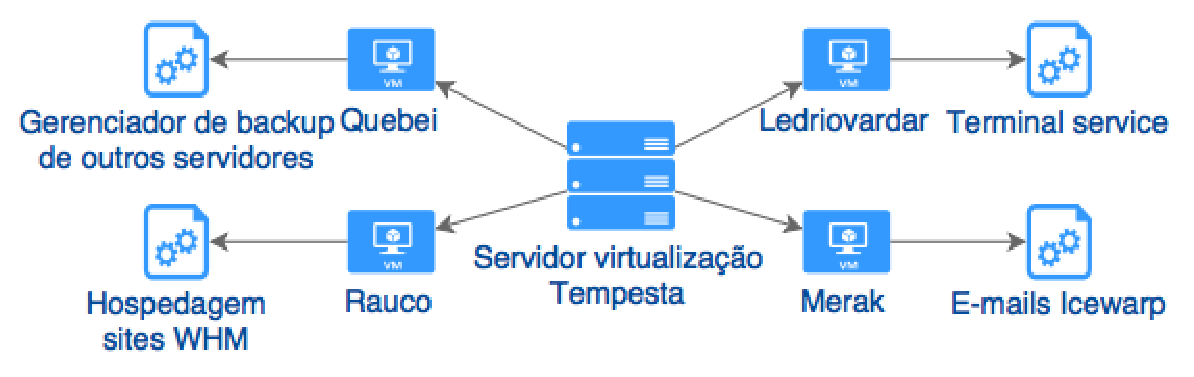
\includegraphics[width=350px]{img/servidor_tempesta.eps}
 \caption{Servidor de virtualização Tempesta.}
 \label{fig:servidor_tempesta}
\end{figure}

\subsection{Servidor Tuono}
\label{section:serv_tuono}

O servidor Tuono possui quatro \ac{VM}s como pode ser visto na Figura \ref{fig:servidor_tuono} juntamente com seus respectivos serviços. 
Esses serviços são listados a seguir:
\begin{itemize}
 \item \textit{Mondoperso}: sua configuração é 1 \textit{core} de processamento, 512 MB de memória e 8 GB de disco. Esse servidor possui o 
 sistema operacional \textit{Ubuntu 14.04 \ac{LTS}} \cite{ubuntu} e fornece \textit{streaming} de áudio para web rádio, esse serviço é feito
 através do \textit{software} livre \textit{Icecast 2.3.3} \cite{icecast};
 
 \item \textit{Ns}: esse servidor possui 1 \textit{core} para processamento, 2 GB de memória e 30 GB de disco. O servidor possui o sistema 
 operacional \textit{CentOS 6.8} \cite{centos} e fornece, através do \textit{software} \textit{Bind 9.9.3} \cite{bind}, o serviço de \ac{DNS} 
 autoritativo e é o servidor de \ac{DNS} primário dos domínios hospedados pela empresa;

 \item \textit{Soldi}: sua configuração é 4 \textit{cores} de processamento, 4 GB de memória e 40 GB de disco. Esse servidor possui o 
 sistema operacional \textit{Ubuntu 14.04 \ac{LTS}} \cite{ubuntu} e é um servidor \textit{web} exclusivo para \textit{softwares} de gestão 
 desenvolvidos pela empresa. Os seguintes \textit{softwares} são utilizados: \textit{Apache 2.4.7} \cite{apache}, \textit{\ac{PHP} 5.5.9} \cite{php} 
 (com \textit{PHP-FPM 5.59}) e \textit{MySQL 5.5.49} \cite{mysql};

 \item \textit{Speedauth}: sua configuração é 2 \textit{cores} para processamento, 1,5 GB de memória e 8 GB de disco. O sistema operacional é o 
 \textit{Ubuntu 14.04 \ac{LTS}} \cite{ubuntu}, sendo que esse servidor fornece o serviço de autenticação \ac{PPPoE} para maior parte dos clientes 
 do provedor utilizando \textit{Radius} (\textit{Freeradius 2.1.12} \cite{freeradius}).
\end{itemize}

\begin{figure}[h!]
 \centering
 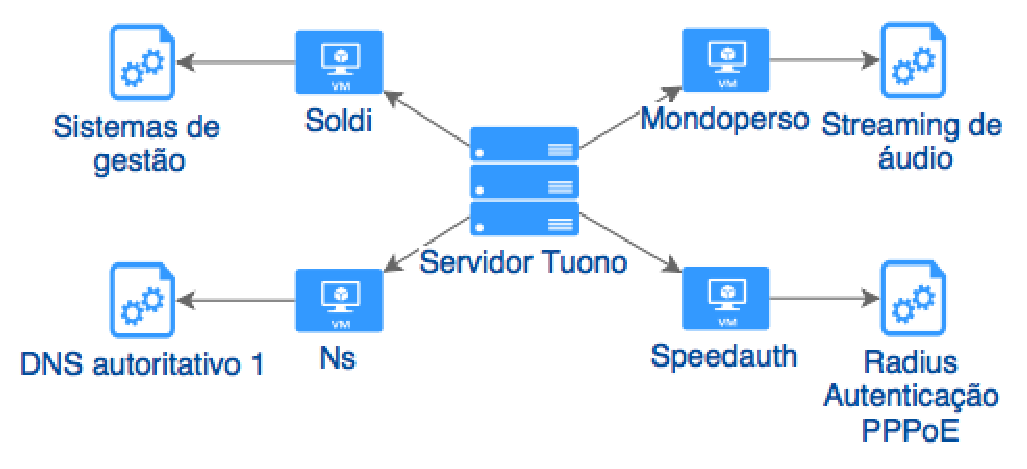
\includegraphics[width=300px]{img/servidor_tuono.eps}
 \caption{Servidor de virtualização Tuono.}
 \label{fig:servidor_tuono}
\end{figure}

\subsection{Servidor Venti}
\label{section:serv_venti}

O servidor Venti possui cinco \ac{VM}s como pode ser visto na Figura \ref{fig:servidor_venti} juntamente com seus respectivos serviços. 
Esses serviços são listados a seguir:
\begin{itemize}
 \item \textit{Backup}: sua configuração é 1 \textit{core} para processamento, 1 GB de memória e 15 GB de disco. Esse servidor possui o 
 sistema operacional \textit{Ubuntu 14.04 \ac{LTS}} \cite{ubuntu} e executa o serviço de \textit{backup} dos equipamentos do provedor. Esse
 utiliza \textit{scripts} que foram desenvolvidos internamente e que buscam e copiam os dados através do protoccolo \ac{FTP};
 
 \item \textit{Esibire}: sua configuração é 1 \textit{core} para processamento, 1 GB de memória e 50 GB de disco. Esse servidor possui o 
 sistema operacional \textit{Ubuntu 14.04 \ac{LTS}} \cite{ubuntu} e faz a hospedagem de vídeos e a reprodução de \textit{streaming} utilizando
 \ac{FTP} e um servidor \textit{web} \textit{Apache 2.4.7};
 
 \item \textit{Miatanto}: sua configuração é 1 \textit{core} de processamento, 1 GB de memória e 8 GB de disco. Esse servidor possui o 
 sistema operacional \textit{Ubuntu 14.04 \ac{LTS}} \cite{ubuntu} e fornece \textit{streaming} de áudio para uma \textit{web} rádio, esse serviço 
 é feito através do \textit{software} livre \textit{Icecast 2.3.3} \cite{icecast};
 
 \item \textit{Pomodoro}: sua configuração é 1 \textit{core} de processamento, 2 GB de memória e 28 GB de disco. Esse servidor possui o 
 sistema operacional \textit{Ubuntu 14.04 \ac{LTS}} \cite{ubuntu} e armazena a documentação dos equipamentos do provedor, utilizando a aplicação
 de código aberto \textit{Sakai 2.9} \cite{sakai};
 
 \item \textit{Trapel}: sua configuração é 1 \textit{core} de processamento, 768 MB de memória e 8 GB de disco. Esse servidor possui o sistema 
 operacional \textit{Ubuntu 14.04 \ac{LTS}} \cite{ubuntu} e fornece um serviço de teste de velocidade da conexão de internet. Os usuários do 
 provedor utilizam esse serviço para testar a velocidade da sua internet. Para isso ele executa as aplicações \textit{Apache 2.4.7} \cite{apache} 
 e \textit{\ac{PHP} 5.5.9} \cite{php}, e um \textit{software} chamado \textit{SpeedTest} \cite{speedtest}.
\end{itemize}

\begin{figure}[h!]
 \centering
 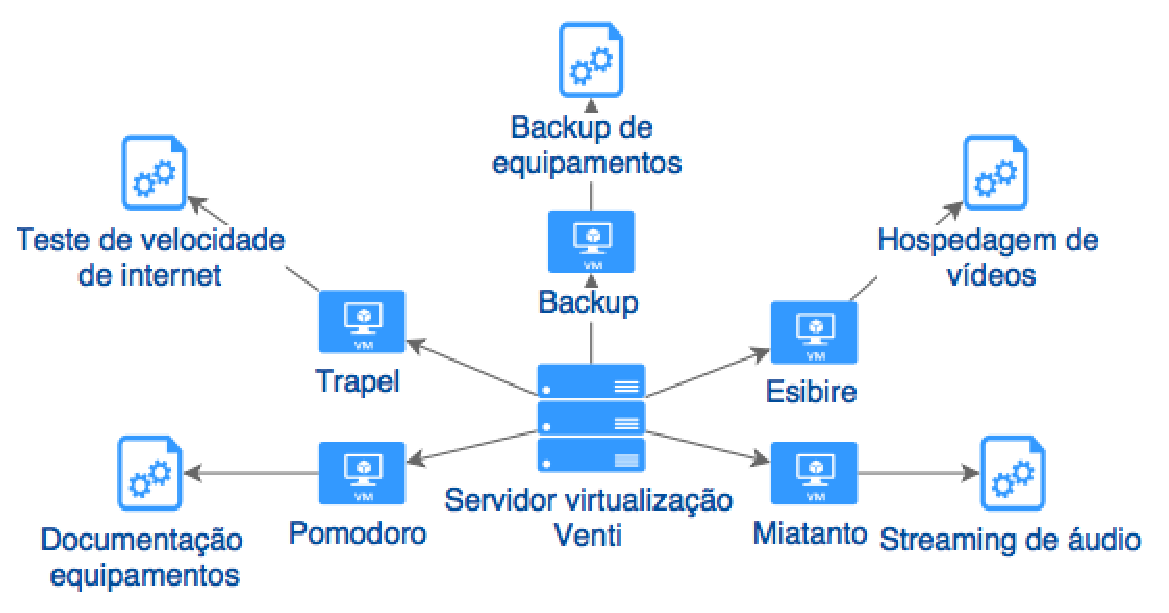
\includegraphics[width=340px]{img/servidor_venti.eps}
 \caption{Servidor de virtualização Venti.}
 \label{fig:servidor_venti}
\end{figure}

-graficos cpu memoria disco cada servidor de virtualizacao?? colocar aqui ou na implementacao??

\section{Serviços críticos}
\label{section:servcrit}

Na seção anterior foram detalhados todos os serviços que estão atualmente disponíveis na empresa. Nesta seção serão descritos os serviços críticos 
para a empresa. Os seguintes critérios serão utilizados para definir os serviços críticos: 
\begin{itemize}
 \item A quantidade de clientes ou funcionários que utilizam o serviço: esse é o item mais relevante, pois impacta diretamente no faturamento
 da empresa. De fato, se um cliente ficar sem acesso à internet, a sua mensalidade é reduzida de acordo com o tempo que ele ficou sem acesso; 
 \item O número de requisições em um determinado tempo: esse número é importante, uma vez que indicam a quantidade de usuários que dependem do 
 serviço. São exemplos dessa medida a quantidade de acessos por minuto em um servidor de hospedagens de sites, ou quantidade de requisições 
 \ac{DNS} em um servidor recursivo;
 \item O volume de objetos do serviço: essa medida demonstra a abrangência do serviço, ou seja, quantos elementos existem em um serviço.
 Como exemplo pode-se citar a quantidade de sites em um servidor de hospedagem, e a quantidade de equipamentos monitorados por um servidor 
 de monitoramento.
\end{itemize}

Considerando esses critérios, foram definidos que os serviços mais críticos são:
\begin{itemize}
 \item \ac{DNS} recursivo primário: esse serviço foi classificado como mais importante pois possui um impacto direto nos clientes do provedor. Esse 
 é o único serviço que todos os clientes utilizam, que totalizam aproximadamente 9000 clientes. O objetivo de um provedor é fornecer uma 
 navegação de qualidade aos seus clientes, sendo assim, o \ac{DNS} é fundamental para essa navegação. Outro importante critério é o 
 número de requisições por segundo (Figura GRAFICO??), que é o maior entre todos os outros serviços;
 
 \item \textit{Radius}: esse serviço também é importante para a navegação dos clientes do provedor, pois, ele faz a autenticação de todos os 
 clientes do provedor. Caso esse serviço fique indisponível os clientes não conseguirão estabelecer conexão para navegação. Esses servidores 
 recebem aproximadamente x?? requisições de autenticação por segundo (Figura GRAFICO FREERADIUS?? 1 e 2). Além disso, esse serviço armazena dados dos 
 clientes: o endereço de \ac{IP} de cada cliente utilizado em um determinado período, o tráfego de dados da conexão, o tempo da conexão de cada 
 cliente, entre outros. Essas operações resultam em um número de requisições por segundo, que esta detalhado nas Figura GRAFICO?? e Figura ;
 
 \item Sistemas da empresa e do provedor: esse serviço não tem um grande impacto direto para os clientes, porém tem um grande impacto para os 
 funcionários da empresa e do provedor. Caso haja uma indisponibilidade dos sistemas a maior parte desses funcionários ficarão 
 impossibilitados de trabalhar (aproximadamente x?? funcionários simultâneos de acordo com a Figura GRAFICO??), isso poderia gerar um prejuizo 
 elevado para a empresa e o provedor. Sendo que o sistema do provedor é responsável pela maior parte das operações do provedor, 
 como por exemplo, emissão de boletos e envio para clientes, atendimento de clientes, comunicação interna da empresa, vendas, 
 ativações de novos clientes, entre outros;
 
 \item Telefonia: esse serviço tem relevância para a empresa e para o provedor, pois permite a comunicação entre clientes e funcionários, 
 e também entre funcionários e outros funcionários, sendo essencial para qualquer empresa. Sabendo que possui uma média de x?? ligações por xx
 (Figura GRAFICO??), sendo que essas ligações são utilizadas por todos o setores do provedor e também da empresa. Exemplos práticos são: 
 atendimento a clientes para suporte técnico, comunicação interna entre funcionários, comunicação com técnicos externos, cobranças a clientes 
 inadimplentes, vendas, entre outros. Levando isso em consideração, se esse serviço ficar indisponível irá gerar prejuízos para a empresa.
\end{itemize}

Tendo esses serviços, pode-se identificar quais máquinas virtuais serão incluídas no ambiente de alta disponibilidade, que são:
\begin{itemize}
 \item \textit{Passata}
 \item \textit{Speedauth}
 \item \textit{Masterauth}
 \item \textit{Soldi}
 \item \textit{SimplesIP}
\end{itemize}

Sendo assim, os recursos das máquinas virtuais, citadas anteriormente, somados são 11 \textit{cores} de processamento, 12 GB de memória e 
156 GB de disco.

-Exibir disponibilidade média atual dos serviços, com gráficos??

\section{Considerações finais}

Neste capítulo foi apresentado a empresa e feito uma análise de seus serviços. Com isso no próximo capítulo será desenvolvido uma proposta 
para implementação de um ambiente de alta disponibilidade nos servidores de virtualização da empresa, além de identificar as ferramentas
que serão utilizadas para essa implementação.


%Esboço: \\
%-DNS (impacto direto para clientes e rede interna): \\
%requisicoes por segundo\\
%numero de usuarios\\
%-Radius (impacto direto para clientes): \\
%numero de usuarios autentidados em x tempo\\
%quantidade de dados armazenados no db em x tempo, tráfego utilizado, tempo conexao\\
%numero de usuarios\\
%-Sistemas (impacto indireto para clientes): \\
%gasto com funcionarios ociosos\\
%quantidade de atendimento a clientes\\
%numero de cobrancas enviadas para clientes efetuar pagamento\\
%comunicacao entre setores e funcionarios\\
%numero de usuarios\\
%-Telefonia (impacto indireto para clientes): \\
%quantidade de atendimento a clientes\\
%comunicacao entre setores e funcionarios\\
%ligacoes saintes, atendimento, cobranca, tecnicos instalacoes internet\\
%numero de usuarios\\


\chapter{Proposta de solução}
\label{cap:propostadesolucao}

Neste capítulo será proposto uma solução de implementação de um ambiente de alta disponibilidade para os serviços críticos da empresa, que 
foram selecionados no capítulo anterior. Com isso pretende-se atingir o objetivo deste trabalho.

O primeiro passo desta implementação é fazer uma reorganização das máquinas virtuais entre os servidores atuais, liberando assim o 
\textit{hardware} suficiente para possibilitar a implementação do ambiente de alta disponibilidade. 

Após ter sido feito a reorganização das máquinas virtuais será iniciado a implementação, montando um ambiente com dois servidores e os 
configurando de uma forma que caso houver alguma falha, em um servidor físico ou no seu sistema operacional hospedeiro, as máquinas serão 
tranferidas para o outro servidor físico. 
A configuração deverá ser: 11 \textit{cores} de processamento, 12 GB de memória e 156 GB de disco para cada servidor. Essa configuração foi 
calculada a partir da soma dos recursos atuais das máquinas virtuais que possuem os serviços críticos, que foram apresentadas no capítulo
anterior na Seção \ref{section:servcrit}.

As ferramentas necessárias para essa implementação podem ser divididas em dois tipos: ferramenta de replicação de dados 
(Seção \ref{section:toolrepl}) e ferramenta que faz o monitoramento e a tranferências das máquinas virtuais em caso de falhas 
(Seção \ref{section:toolcluster}).

\section{Ferramentas de replicação de dados}
\label{section:toolrepl}

Replicação de dados pode ser feita de diversas maneiras, pode ser a nível de aplicação ou até mesmo a nível de \textit{hardware}.
Dependendo do objetivo e da aplicação pode-se usar ferramentas como por exemplo o \textit{rsync}, que faz o sincronismo de dados de uma origem
para um destino. Sendo assim, não é possível utilizar essa ferramenta, pois ela não faz a replicação em tempo real, ou seja, se for necessário
utilizar os dados de destino ocorrerá perda de dados. Outra forma de replicação é a de discos com \ac{RAID} por exemplo, essa solução é eficaz
para garantir que o sistema não fique indisponível em caso de falha de discos\footnote{Lembrando que essa solução é utilizada no ambiente atual
para aumentar a disponibilidade dos servidores}, porém não garante a disponibilidade quando algum componente de \textit{hardware} falhar 
\cite{zaminhani2008}.

A solução de replicação ideal para esta implementação é um espelhamento de dados através da redes, assim permitindo a cópia dos dados para uma
máquina remota. Essa solução além de fazer a replicação dos dados, faz a redundância de todo \textit{hardware}.

A ferramenta escolhida para replicação de dados na solução de alta disponibilidade desse trabalho foi o \ac{DRBD}. Essa ferramenta é de código
aberto, e permite a replicação de dados de um dispositivo local em tempo real. 
APROFUNDAR AQUI OU NA IMPLEMENTAÇÂO?

% dispositivo primario e secundario zaminhani2008
% Segundo (ELLENBERG, 2007), a partir da versão 8 do DRBD é possível que,
%dependendo da aplicação, a execução ocorra em todos os nós do cluster
%simultaneamente (Ativo/Ativo). Para tornar isso possível é necessária a
%utilização de um sistema de arquivos exclusivo para cluster, como o OCFS2 6 e o
%GFS 7 por exemplo. Como a abordagem deste trabalho é cluster de alta
%disponibilidade, a utilização do DRBD no modo Ativo/Ativo não será discutida.

\section{Ferramentas de gerenciamento de cluster}
\label{section:toolcluster}

Para ser possível implementar uma solução de alta disponibilidade é necessário uma ferramenta que monitora os recursos, fazendo a detecção e
recuperação do serviço utilizando mensagens entre os servidores \cite{perkov2011}.

Definir clusteer...

\textit{Pacemaker} é uma ferramenta de detecção e recuperação de falhas a nível de serviço \cite{perkov2011}. Essa ferramenta é um projeto da
xx, ele é classificado como um CRM...
Continuar ??? \textit{Heartbeat} ou \textit{Corosync} \cite{zaminhani2008}.

cluster resource manager (CRM) which has the task of starting and stopping the services (IP addresses, web servers, etc)


Explicar live migration \ref{fig:vms_migration}
%http://www.aliancatecnologia.com/conteudo/2015/05/quatro-estrategias-de-protecao-para-seu-ambiente-virtual/

\begin{figure}[h!]
 \centering
 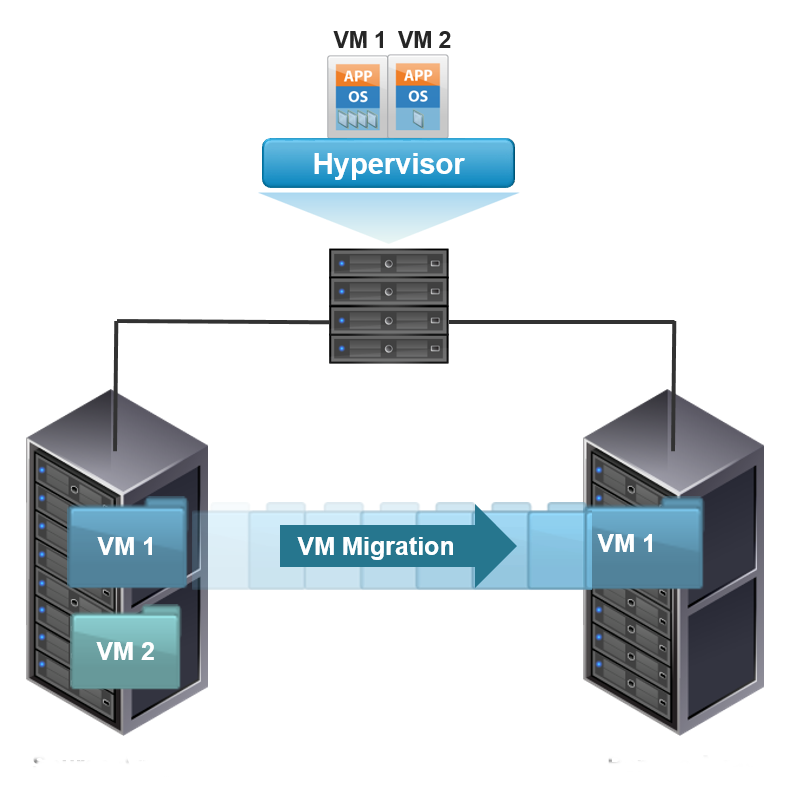
\includegraphics[width=300px]{img/vms_migration.eps}
 \caption{Live migration}
 Fonte: \citet{spaniol2015}
 \label{fig:vms_migration}
\end{figure}


%reorganização de vms
%ferramentas selecionadas, colocar motivo para escolher e citar ferramentas parecidas
%muitos servicos, melhor solucao utilizar 2 servidores para fazer redundancia
%em caso de falha de um servidor fisico...
%ferramentas open source...
%colocar a disponibilidade do nagios do ano passado?

\chapter{Implementação e resultados}
\label{cap:implementacaoresultados}

Neste capítulo será detalhado a implementação, com a configuração do \ac{OS}, do ambiente virtualizado e das ferramentas que irão compôr o
\textit{cluster} de alta disponibilidade. Posteriormente, serão efetuados testes e medições.

Descrever o que nao deu certo no projeto?

\section{Topologia}


\section{Configuração do \ac{OS}}


\section{Configuração de rede}


\section{Configuração de disco}


\section{Configuração do ambiente virtualizado}


\section{Configuração do cluster}


\chapter{Conclusão}
\label{cap:conclusao}

Neste trabalho foi feito um estudo sobre uma empresa prestadora de serviços para Internet, analisando sua estrutura física e os serviços oferecidos 
por essa. Durante este estudo foram definidos os serviços críticos. Para tanto considerou-se o impacto dos mesmos para a empresa, medido através
da quantidade de clientes e funcionários que utilizam o serviço. Destaca-se que foi necessário selecionar os serviços mais críticos, por não 
haver recursos necessários para implementar a alta disponibilidade para todos os serviços.

Deste modo, os serviços críticos definidos foram: o serviço de \ac{DNS} recursivo, pois é utilizado para navegação de Internet de todos os clientes 
e funcionários do provedor; o serviço de autenticação \textit{Radius}, por influenciar diretamente na navegação dos clientes e armazenar dados 
importantes para o provedor; sistemas da empresa, uma vez que todos os funcionários o utilizam e também por ter um impacto indireto nos 
clientes; e serviço de telefonia interna, por ser responsável pela comunicação tanto entre funcionários, como entre clientes e funcionários.

Após implementou-se um ambiente de alta disponibilidade para esses serviços. Esse ambiente é composto por um \textit{cluster} o qual é constituído 
por dois servidores físicos. Para o gerenciamento do \textit{cluster} foi adotado o \textit{software} \textit{Pacemaker}, que é responsável pelo 
monitoramento e a transferência das máquinas virtuais, as quais executam os serviços. Para a replicação de dados 
do \textit{cluster} foi adotado o \textit{software} \ac{DRBD}, que é responsável pela replicação dos dados entre os dois servidores.

O ambiente de alta disponibilidade é composto por máquinas virtuais que executam os serviços críticos. Para garantir a disponibilidade 
foi utilizada a opção de migração em tempo real, fornecida pelo hipervisor \ac{KVM}, juntamente com o \textit{Pacemaker}. Desta forma, 
caso seja necessário fazer uma manutenção em um dos servidores, as máquinas virtuais serão migradas para o outro servidor.
Além disso, caso um servidor falhe, as máquinas virtuais serão automaticamente iniciadas no outro servidor, diminuindo assim a indisponibilidade
dos serviços e o impacto para a empresa.

De fato, os testes realizados mostraram que em casos de falhas de \textit{hardware}, de energia elétrica ou de \textit{software}, 
o \textit{cluster} conseguiu recuperar os serviços executados nas máquinas virtuais. Além disso, o ambiente de alta disponibilidade possibilitou
realizar manutenções previamente agendadas sem gerar indisponibilidade para os serviços.
Foi possível analisar a comparação de disponibilidade feita entre o ambiente de alta disponibilidade implementado e o antigo ambiente,
e perceber que houve uma melhora na disponibilidade. 
Desta forma, conclui-se que é possível aumentar a disponibilidade de serviços em máquinas virtuais utilizando uma solução 
de código aberto e de baixo custo.
Conclui-se também que em caso de uma falha permanente de um \textit{hardware}, os dados permanecerão íntegros e disponíveis, assim garantindo 
uma maior segurança dos dados e informações da empresa.


\section{Trabalho futuros}
\label{section:trabalhosfuturos}

Com a implementação apresentada neste trabalho pode-se perceber a variedade de ferramentas existentes para implantar soluções de alta 
disponibilidade. Deste modo, pode-se testar outras ferramentas de alta disponibilidade. Assim, sugere-se que seja feito um estudo de
viabilidade do uso das ferramentas como \textit{GlusterFS} e \textit{Ceph}, em conjunto com uma ferramenta de gerenciamento de nuvem, como
por exemplo, o \textit{OpenStack}, que trarão mais alguns benefícios além da alta disponibilidade.
Além disso, sugere-se a inclusão de todos os serviços da empresa neste ambiente. De fato, pretende-se fazer a inclusão de mais alguns
serviços com nível de criticidade médio.
Por fim, pode-se efetuar uma medição de disponibilidade por um período mais longo, a fim de se certificar sobre o aumento da
disponibilidade.



\bibliography{tcc}
\bibliographystyle{abnt}

\end{document}
